\documentclass[11pt,letterpaper]{article}
%\pdfoutput=1
\usepackage{mathtools}
\usepackage{axodraw2}
\usepackage{tikz}
\usepackage{tikz-feynman}
\usepackage{amscd}
\usepackage{amsmath}
\usepackage{slashed}
\usepackage{gensymb}
\usepackage{bm}
\usepackage{jheppub} % for details on the use of the package, please
\usepackage{booktabs}
\usepackage{array}  
\usepackage[capitalise]{cleveref}
\usepackage{comment}
\usetikzlibrary{shapes.misc}

\newcommand{\model}{Plan B Model}
\newcommand{\bsll}{$b \rightarrow s \ell^+ \ell^-$}
\newcommand{\bsmm}{$b \rightarrow s \mu^+ \mu^-$}
\newcommand{\bsee}{$b \rightarrow s e^+ e^-$}

\newcommand{\bca}[1]{\textcolor{blue}{BCA: #1}}
\newcommand{\pcs}[1]{\textcolor{red}{PCS: #1}}

\title{\centering
% Uncomment closer to the time of publication
Neutrino masses and mixing angles in the \model}

\author[a]{Ben Allanach}
\affiliation[a]{DAMTP, University of Cambridge, Wilberforce Road, Cambridge, 
  CB3 0WA, United Kingdom}
\emailAdd{ben.allanach.work@gmail.com}

\author[1]{and Prabhoda Chandra Sarjapur\note{Corresponding author.}}
\emailAdd{prabhodacs@gmail.com}

\abstract{The Plan B Model is based on applying an additional
  spontaneously broken  $U(1)_{3B_3-L_1-2L_2}$
  gauge symmetry to the Standard Model (SM) with family-dependent
  fermion charges. Right-handed neutrino fields are present and cancel gauge anomalies. The model was proposed
  to ameliorate fits of the SM to observables 
  involving the $b\rightarrow s l^+ l^-$ transition whilst simultaneously
  explaining the relatively large mass of the third family of quarks, compared
  to the first two. 
  We investigate its implications for neutrino masses and mixing angles.
  The \model\ naturally implements the Froggatt-Nielsen mechanism for neutrino
  mass and mixing hierarchies via a Type-I see-saw mechanism. 
  One or two apparently fundamental Yukawa couplings must be suppressed beyond
  the Froggatt-Nielsen model in order to fit neutrino oscillation data well:
  we give examples of how this might be 
  achieved via a clockwork extension of the model in an appendix. 
}   

\keywords{$B-$anomalies, beyond the Standard Model, flavour changing neutral
  currents, neutrino masses}

\begin{document} 

\maketitle
\flushbottom

\section{Introduction \label{sec:intro}}

Various measurements of $B-$meson decays at LHC experiments are in tension
with state-of-the-art SM predictions, particularly when there is a bottom to
strange flavour transition accompanied by a di-lepton (i.e.\ di-electron or
di-muon) pair.
Measurements in several di-muon invariant mass-squared ($q^2$)
bins of the branching ratio of the $B_s$ meson decaying to a $\phi$ meson and
a di-muon pair
$BR(B_s \rightarrow \phi \mu^+ \mu^-)$ are up to $4\sigma$ smaller than the SM
predictions~\cite{LHCb:2021zwz,CDF:2012qwd}.
Some angular distributions in $B \rightarrow K^\ast \mu^+ \mu^-$
decays have been measured by LHC
experiments~\cite{LHCb:2013ghj,ATLAS:2018gqc,CMS:2017rzx,CMS:2015bcy,Bobeth:2017vxj}
to be several $\sigma$ short of state-of-the-art SM
predictions and
the same can be said of $BR(B \rightarrow K^\ast \mu^+
\mu^-)$~\cite{Parrott:2022zte}. On the other hand, many measurements agree with the
prediction of the SM (to
within 1$\sigma$ or so), for example lepton flavour universality in $b \rightarrow s
l^+ l^-$ transitions\footnote{When we mention \bsll\ transitions, we
implicitly include the $CP$ conjugate mode $\bar b \rightarrow \bar s l^+
l^-$.}~\cite{LHCb:2022qnv} and SM predictions of $B_s-{\overline{B_s}}$ mixing~\cite{PDG}.
In Ref.~\cite{Allanach:2023uxz}, it was shown that the so-called \model\ can
significantly ameliorate a global fit of the SM to flavour observables via the predicted
family non-universal 
interactions of the model's TeV-scale $Z^\prime$ vector boson; the total $\chi^2$ (of
hundreds of observables) improved by 34 units in the model, which has only two
effective fit parameters. 
The best-fit point (BFP) simultaneously
satisfies experimental constraints from di-lepton production at LEP2, which receives contributions
from an intermediate tree-level off-shell $Z^\prime$ boson. Current LHC bounds upon
direct searches for
the $Z^\prime$ are rather modest: $M_{Z^\prime} > 1.2$~TeV~\cite{Allanach:2024jls} in the parameter range that is compatible with both perturbativity and the global fit. 

The \model\ augments the gauge Lie algebra of the SM by a $u(1)_X$ summand additional to that of $u(1)$ hypercharge in the SM. The charges of the SM Weyl fermionic quantum fields are assigned to be equal to thrice third family baryon number minus first family lepton number minus twice second family lepton number:
\begin{equation}
X = 3B_3-L_1-2L_2.    
\end{equation}
In order to allow a renormalisable top quark Yukawa coupling, the Higgs $X$
charge is fixed to vanish. This is necessary because the top quark Yukawa
coupling is the largest dimensionless parameter in the SM Lagrangian at the
electroweak scale (its value is 1); as we shall see below, one can induce
smaller Yukawa couplings by banning them at the renormalisable level with a
symmetry but inducing them through spontaneous symmetry breaking. The
additional $u(1)_X$ is spontaneously broken by a SM-singlet complex scalar
field, the `flavon' $\theta$, which is assumed to have an $X$ charge of unity
and acquire a TeV-scale vacuum expectation value (VEV), leading to a TeV-scale
$Z^\prime$ vector boson with family-dependent gauge couplings. At the
renormalisable level, the  Yukawa couplings have the texture (where here and
later in the paper, $\times$ indicates a non-zero entry)
\begin{equation}
    Y_U , Y_D \sim \begin{pmatrix}
    \times & \times & 0 \\
        \times & \times & 0 \\      
        0 & 0 & \times
    \end{pmatrix}, \qquad
    Y_E \sim \begin{pmatrix}
    \times & 0 & 0 \\
        0& \times & 0 \\      
        0 & 0 & \times
    \end{pmatrix}. \label{chferms}
\end{equation}
At this renormalisable level, charged lepton flavour violation is then banned. 
Charged lepton flavour violation (CLFV) is heavily constrained by searches for it, especially in the $\mu \rightarrow e \gamma$ channel~\cite{MEGII:2023ltw}.
(\ref{chferms}) predicts zero values for the magnitudes of Cabbibo-Kobayashi-Maskawa (CKM) matrix elements $|V_{ub}|,|V_{cb}|,|V_{td}|$ and $|V_{ts}|$, whereas $|V_{us}|$ and $|V_{cd}|$ are generically predicted to be of order unity. The spontaneous breaking of $u(1)_X$ will generically predict that instead of zeroes, the CKM matrix elements are instead merely much smaller than unity, a feature which agrees with measurements~\cite{PDG}. 

The Froggatt-Nielsen (FN) mechanism~\cite{Froggatt:1978nt} constitutes a suggestion as to where smaller Yukawa couplings could originate (following $u(1)_X$ spontaneous symmetry breakdown). The idea that there are some fermionic fields which are in vector-like representations of the SM gauge symmetry with masses above the scale $\langle \theta \rangle$ of $u(1)_X$ breaking.
Let us call this mass scale $\Lambda_{\text{FN}} \gg \langle \theta \rangle$. For the Yukawa couplings constrained to be zero at the reonormalisable level, after $u(1)_X$ symmetry breaking, the dominant contribution to the effective Yukawa coupling term of the Lagrangian density between SM Weyl fermion $\psi_i$ and SM Weyl fermion $\psi_j$ and the Higgs doublet field H is assumed to be 
\begin{equation}
    {\mathcal L}_{\overline{\psi_i} H \psi_j} = A \overline{\psi_i} H \psi_j  \left( \frac{\langle \theta \rangle}{\Lambda_{\text{FN}}}\right)^{X_i-X_j},
    \label{effop}
\end{equation}
where $X_i$ is the $X$ charge of the Weyl fermionic field labelled by $i$ and $A$ is a product of (presumably) order unity dimensionless couplings of some underlying ultra-violet theory, of which we shall hear more of below.  The number of powers of $\theta$ in the numerator fixes the Lagrangian density operator to be $U(1)_X$ group invariant and, depending on $X_i-X_j$, provides varying levels of suppression of the effective Yukawa coupling. 
The idea is that the operator in (\ref{effop}) would be generated by underlying renormalisable physics in the ultra-violet, for example by the ``spaghetti diagram" in Fig.~\ref{fig:spag}.


\begin{figure}[t] 
    \centering
    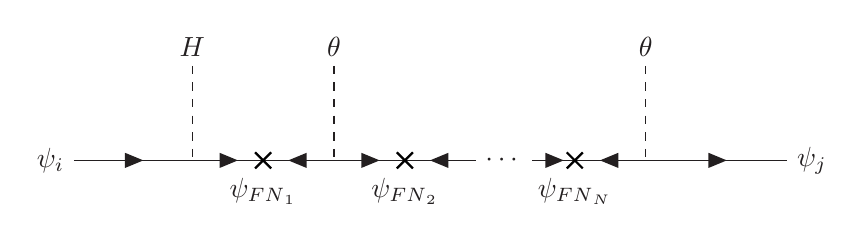
\begin{tikzpicture}
        \begin{feynman}
            \vertex (L) {$\psi_i$};
            \vertex [right=1.8cm of L] (F1);
            \vertex [right=0.9cm of F1] (G1);
            
            \vertex [right=0.9cm of G1] (F2);
            \vertex [right=0.9cm of F2] (G2);
            \vertex [right=0.9cm of G2] (dots) {$\cdots$};
            \vertex [below=0.1cm of G1] (FN1) {$\psi_{{FN}_1}$};
            \vertex [below=0.1cm of G2] (FN2) {$\psi_{{FN}_2}$};

            \vertex [right=0.9cm of dots] (GN);
            \vertex [right=1.8cm of dots] (FN);

            \vertex [below=0.1cm of GN] (FN3) {$\psi_{{FN}_N}$};       
            
            \vertex [right=1.8cm of FN] (R) {$\psi_j$};

            \vertex [above=1.2cm of F1] (phi1) {$H$};
            \vertex [above=1.2cm of F2] (phi2) {$\theta$};
            \vertex [above=1.2cm of FN] (phiN) {$\theta$};

            \diagram*{
            (L) -- [fermion] (F1),
                
            (F1)-- [fermion] (G1),
            (F2)-- [fermion] (G1),   
            
            (F2)-- [fermion] (G2),
            (dots)--[fermion] (G2),
            
            (dots)-- [fermion] (GN),
            (FN)-- [fermion] (GN),
                
            (FN)-- [fermion] (R),

            (phi1) -- [scalar] (F1),
            (phi2) -- [scalar] (F2),
            (phiN) -- [scalar] (FN),
            };
            \node [cross out, draw=black, thick, minimum size=5pt, inner sep=0pt] at (G1);
            \node [cross out, draw=black, thick, minimum size=5pt, inner sep=0pt] at (G2);
            \node [cross out, draw=black, thick, minimum size=5pt, inner sep=0pt] at (GN);
        \end{feynman}
    \end{tikzpicture}
    \caption{The ``spaghetti'' Feynman diagram leading to an approximate effective field theory FN operator $A\left(\frac{\langle\theta \rangle}{\Lambda_{\text{FN}}} \right)^{X_i-X_j} \overline{\psi_i} H \psi_j$. Each $\times$ represents a mass insertion of a different heavy beyond-the-SM fermionic field $\psi_{\text{FN}_i}$ whose charges are integers, differing by one unit in each case from left to right. $\psi_{\text{FN}_i}$ are in vector-like representations of the SM gauge group and have mass scale $\Lambda_{\text{FN}}$. $A$ is an effective coupling given by the product of all couplings in the diagram and another factor taking into account any mass-splitting between the $\psi_{\text{FN}_i}$ fields.}
    \label{fig:spag}
\end{figure}

In order to cancel gauge anomalies, the \model\  augments the SM Weyl fermionic field content by three right-handed neutrino type fields~\cite{Allanach:2023uxz}, i.e. SM-gauge-singlet right-handed Weyl fermionic fields but with $X$ charges  $-1$, $-2$ and $0$, respectively\footnote{Strictly speaking, the right-handed neutrino with $0$ $X$-charge is not required for gauge anomaly cancellation; it is added for aesthetic reasons.}. Such right-handed neutrinos have the potential to implement the see-saw mechanism~\cite{Yanagida:1980xy}, which suppresses Dirac neutrino masses by a heavy neutrino mass scale in order to explain why neutrinos have such small masses compared to the other observed SM fermionic fields via the dimension-4 Lagrangian density terms
\begin{equation} \label{Neutrino Mass Lagrangian}
  {\mathcal L} = \ldots - {\overline L_i} (Y_\nu)_{ij} \tilde{H} \nu_{R_j} - \frac{1}{2}
  {\overline{(\nu_{R_i})^c}} M_{ij} \nu_{R_j} + \textrm{H.c.},
  \end{equation}
where $i,j \in \{1,2,3\}$ are family indices (with an implied Einstein summation convention on repeated indices) and gauge indices have been suppressed. $(Y_\nu)_{ij}$ is a matrix of dimensionless Yukawa couplings and $M_{ij}$ is a matrix of mass-dimension 1 Majorana masses.

After spontaneous electroweak symmetry breaking, we can write the Higgs field as $H = (0, (v+h)/\sqrt{2})^T$ (where $h$ is now a real scalar field) and generate mass-like terms for the neutrinos through the Yukawa terms. Combining this with the Majorana terms and writing vectors in flavour space in bold font,
\begin{equation}
    \bm{\nu}_L =
    \begin{pmatrix}
        \nu_{eL} \\ \nu_{\mu L} \\ \nu_{\tau L}
    \end{pmatrix}
\end{equation}
we can rewrite \cref{Neutrino Mass Lagrangian} as 
\begin{equation}
    \mathcal{L}_\nu \supset - \frac{1}{2}\begin{pmatrix}
        \overline{\bm{\nu}_L} & \overline{\bm{\nu}_R^c}
    \end{pmatrix} \bm{M}_\nu \begin{pmatrix}
        \overline{\bm{\nu}_L^c} \\ \overline{\bm{\nu}_R}
    \end{pmatrix},
\end{equation}
where $\bm{M}_\nu$ is a 6 by 6 complex symmetric matrix
\begin{equation} \label{neutrino mass matrix}
    \bm{M}_\nu = \begin{pmatrix}
        0 & m_{\nu D} \\
        m_{\nu D}^T & M
    \end{pmatrix}
\end{equation}
and $m_{\nu D} = v\bm{Y}_\nu/\sqrt{2}$, where $\bm{Y}_\nu$ is the 3 by 3 matrix with entries $Y_{\nu_{ij}}$. If the non-zero entries in the Majorana mass matrix are much greater than the electroweak scale $M_{ij} \gg v$, we can use matrix perturbation theory. Then, the three right-handed neutrinos have a mass matrix $m_{\nu R} \approx M$ and the three  left handed neutrinos having the mass matrix~\cite{gell-mann_complex_2013, minkowski_e_1977, glashow_future_1980}.
\begin{equation}
m_{\nu L}\approx -\frac{1}{2}m_{\nu D}^T M^{-1} m_{\nu D}. \label{mnu_eff}
\end{equation}
The suppression by $M^{-1}$ explains the lightness of the approximately left-handed neutrino mass eigenstates, whereas the large mass scales present in the right-handed neutrino masses lead to heavy right-handed neutrino mass eigenstates. 

In the \model, we already have right-handed neutrinos as well as a $U(1)_X$ symmetry that potentially implements the FN mechanism. It is natural then to see if the FN mechanism can be made to work in a simple way that agrees with measurements of neutrino oscillations and constraints upon neutrino mass in detail utilising the Type I see-saw mechanism. \emph{This is the central purpose of our paper}. We will show how an inverted neutrino mass spectrum can be obtained quite naturally, whereas a hierarchical one requires the percent-level suppression of a coupling that one might normally expect to be of order unity. In order to present this analysis, we first display the neutrino mass spectrum at the renormalisable level (in terms of the SM plus right-handed neutrinos) in \S\ref{sec:origin}. Then we display neutrino  neutrino mass matrices in \S\ref{sec:offdiag}, analytically studying them using perturbation theory in \S\ref{sec:anal}. We then present the normal hierarchy case in \S\ref{sec:Normal Hierarchy} and the inverted hierarchy case in \S\ref{sec:Inverted Hierarchy}. Because the normal hierarchy case requires a further suppression of a coupling beyond the FN mechanism, we detail a potential clockwork-like mechanism to implement it in Appendix~\ref{Sec:Clockwork}. We summarise and conclude in \S\ref{sec:conc}.

\section{Origin of neutrino masses and lepton mixing} \label{sec:origin}
\begin{comment}
The \model\  augments the gauge symmetry of the SM by an additional $U(1)_X$
factor, where the $U(1)_X$ family-dependent fermionic field charges are fixed
to be three times third family baryon number minus electron number, minus
twice muon number. In order for the model to be free of quantum field
theoretic anomalies, one requires it to contain at least two further
right-handed neutrino $\nu_{R_{1,2}}$ fields. A third, $\nu_{R_3}$, is added so that the
three families of fermionic fields are identical from the point of view of the SM symmetries. This $U(1)_X$ symmetry is broken by the complex scalar field dubbed the flavon, $\theta$, at the TeV scale ($\langle \theta \rangle \sim \mathcal{O}(\text{TeV})$).
\end{comment}
\begin{comment}
    While the primary motivation for the \model was to resolve B-meson decay anomalies, given its family-dependent charge structure, it also displays a great adaptive power in explaining the mass matrix structures of both the quark \cite{Allanach:2023uxz} and lepton sectors. 
\end{comment}

\begin{table}[ht]
\centering
\setlength{\tabcolsep}{10pt}     % horizontal padding
\renewcommand{\arraystretch}{1.2}  % vertical padding
\begin{tabular}{|c|c|c|c|c|c|}
    \hline
     & $L_1, \,\, L_2, \,\, L_3$ & $e_1, \,\, e_2, \,\, e_3$ & $\nu_1, \,\, \nu_2, \,\, \nu_3$& $H$ &$\theta$\\
    \hline
    $SU(3)$ & $\bm{1}$ & $\bm{1}$ & $\bm{1}$ & $\bm{1}$ & $\bm{1}$ \\
    $SU(2)$ & $\bm{2}$ & $\bm{1}$ & $\bm{1}$ & $\bm{2}$ & $\bm{1}$ \\
    $U(1)_Y$ & -3 & -6 & 0 & 3 & 0 \\
    $U(1)_X$ & $-1, \,\, -2, \,\, 0$  & $-1, \,\, -2, \,\, 0$ & $-1, \,\, -2, \,\, 0$ & 0 & 1 \\
    \hline
\end{tabular}
\caption{Lepton and scalar field charge assignments under 
$SU(3)\!\times\!SU(2)\!\times\!U(1)_Y\!\times\!U(1)_X$. $L_i$ are left-handed Weyl fermion fields, whereas the rest of the fields are right-handed, and $H$ and $\theta$ are the complex scalar Higgs doublet and the complex scalar flavon, respectively.}
\label{tab:lepton_charges}
\end{table}

While the primary motivation for the \model\  was to resolve $B$-meson decay anomalies, the model necessarily includes right-handed neutrino fields, making the neutrino sector of interest for study. As explained in \S\ref{sec:intro}, we wish to see if the $U(1)_X$ symmetry is compatible with neutrino masses and mixing parameters which agree with those extracted from neutrino oscillation phenomena via the FN mechanism as well as suppressing CLFV.

\begin{comment}
    the same texture induced by the \model\ which suppresses off-diagonal terms in \cref{chferms} for the charged-lepton sector could also be used to generate controlled, hierarchical entries in the neutral-lepton sector with the FN mechanism to test the model's predictions. \bca{I disagree with this sentence. It's not the charged fermion \emph{texture} that does it. Suggest to replace with: "As explained in \S\ref{sec:intro}, we wish to see that if the $U(1)_X$ symmetry can generate neutrino masses and mixing parameters which agree with those extracted from neutrino oscillation phenomena via the FN mechanism as well as suppressing CLFV."}
    
However, due to precision experiments on neutrino oscillations \cite{ParticleDataGroup:2024cfk} (given in \cref{tab:neutrino_angles_masses}), we know this not to be the case. 
\bca{Replace last sentence with "These predictions  (given in \cref{tab:neutrino_angles_masses}) are incompatible with precision experiments on neutrino oscillations \cite{ParticleDataGroup:2024cfk}."}

\end{comment}

At the renormalisable level, ${Y}_\nu$ and ${M}$  are diagonal by virtue of them remaining invariant under the $U(1)_X$ charge assignment given in \cref{tab:lepton_charges}.
\begin{equation} \label{renormalizable Y and M}
    Y_{\nu}  \sim  
    \begin{pmatrix}
    \times & 0 & 0 \\
    0 & \times & 0 \\
    0 & 0 & \times 
    \end{pmatrix}, \,\,\,\,\,\,
    M  \sim 
    \begin{pmatrix}
    0 & 0 & 0 \\
    0 & 0 & 0 \\
    0 & 0 & \times 
    \end{pmatrix},
\end{equation}
which would imply no neutrino mixing and two massless right-handed neutrinos. These predictions are incompatible with experimental inference (given in \cref{tab:neutrino_angles_masses}) from neutrino oscillation phenomena~\cite{ParticleDataGroup:2024cfk}. In the basis where the charged lepton matrix is diagonal, which is natural for the \model, the Pontecorvo–Maki–Nakagawa–Sakata (PMNS) matrix arises solely due to the misalignment of the neutrino sector between the gauge and mass eigenbasis, i.e.,
\begin{equation} \label{eqn:PMNSdefn1}
    \begin{pmatrix}
        \nu_{eL} \\ \nu_{\mu L} \\ \nu_{\tau L} 
    \end{pmatrix} = U_{PMNS} \begin{pmatrix}
        \nu_{1L} \\ \nu_{2 L} \\ \nu_{3 L} 
    \end{pmatrix},
\end{equation}
where 
\begin{equation} \label{eqn:PMNSdefn2}
    \text{diag}(m_1, m_2, m_3) = U_{PMNS}^\dagger m_{\nu L} U_{PMNS}^*
\end{equation}
To explain the mass hierarchy and the PMNS matrix, one must go beyond the renormalisable level of the Lagrangian and include symmetry-permitted higher-dimensional operators suppressed by the heavy scale $\Lambda_{\text{FN}}$ to the off-diagonal entries in \cref{renormalizable Y and M}. The presence of such higher dimensional operators is natural from the point of view of UV completions of the model, and is the defining feature of FN models \cite{froggatt_hierarchy_1979}.
\begin{table}[ht]
\centering
\setlength{\tabcolsep}{10pt}
\renewcommand{\arraystretch}{1.3}
\begin{tabular}{@{} l c c @{}}
    \toprule
    & \multicolumn{2}{c}{\textbf{Experimental Values ({\tt NuFIT 6.0})} \cite{esteban_nufit-60_2024}} \\
    \cmidrule(l){2-3} 
    \textbf{Parameter} & Normal Ordering & Inverted Ordering \\
    & (Best Fit $\pm 1\sigma$) & (Best Fit $\pm 1\sigma$) \\
    \midrule
    $\theta_{12}/^\circ$ & $33.68^{+0.73}_{-0.70}$ & $33.68^{+0.73}_{-0.70}$ \\
    $\theta_{23}/^\circ$ & $43.3^{+1.0}_{-0.8}$ & $47.9^{+0.7}_{-0.9}$ \\
    $\theta_{13}/^\circ$ & $8.56^{+0.11}_{-0.11}$ &  $8.59^{+0.11}_{-0.11}$  \\
    $\Delta m_{21}^2/10^{-5}\text{eV}^2$ & $7.49^{+0.19}_{-0.19}$ & $7.49^{+0.19}_{-0.19}$\\
    $\Delta m_{3l}^2/10^{-3}\text{eV}^2$ & $+2.513^{+0.021}_{-0.019}$ & $-2.484^{+0.020}_{-0.020}$\\
    \hline
\end{tabular}
\caption{Three-flavour neutrino oscillation data as of Sept 2024 (including data from the Super Kamiokande (SK) experiment) \cite{esteban_nufit-60_2024}. Normal ordering corresponds to $\Delta m_{3l}^2=\Delta m_{31}^2>0$ and  inverted ordering to $\Delta m_{3l}^2 = \Delta m_{32}^2<0$. 
The leptonic mixing angles (parameterising
the PMNS matrix) are defined in Eq.~(14.33) of Ref.~\cite{PDG}.}
\label{tab:neutrino_angles_masses}
\end{table}
\begin{comment}
\bca{I suspect that we also want to put a column with the experimental estimates of these quantities in a column of this table, along with a citation. } \pcs{This table are expetrimental values taken entirely from \cite{esteban_nufit-60_2024}

\bca{Detail values for neutrino mass squared differences and mixing angles extracted from the PDG that we are using for our fits in a table.}

        \section{Neutrino masses}
    the Yukawa and Majorana matrices are diagonal by virtue of remaining invariant under the new gauge group charges,
    
    The neutrino mass matrix has the form
    \begin{equation} \label{Full neutrino mass matrix}
        M_\nu = \begin{pmatrix}
            0 & m_{\nu D} \\ m_{\nu D}^T & M_R 
        \end{pmatrix},
    \end{equation} 
    where $m_{\nu D} = \frac{v}{\sqrt{2}} Y_\nu$ and $M_R$ is a complex, symmetric $3 \times 3$ matrix, whose eigenvalues $(M_1, M_2, M_3)$ are the three heavy neutrino masses.
    
    For the LH neutrino masses, we get: $m_\nu = m_{\nu D} M_R^{-1}m_{\nu D}^T = \frac{v^2}{2} Y_{\nu} M_R^{-1}Y_{\nu}^T$. For the charged lepton sector, we get $Y_e$ diagonal too, with the current bounds on $\mu \rightarrow e \gamma$ \cite{navas_review_2024} enforcing close to zero off-diagonal terms. This further implies that to go from the mass eigenbasis to the weak eigenbasis, one needs only the similarity transform matrix that diagonalizes the $m_\nu$ matrix, that is, $U_{PMNS} = V^\dagger_{\nu_L}$.
\end{comment}

\subsection{Off-Diagonal entries and the Froggatt-Nielsen Mechanism} \label{sec:offdiag}
\begin{comment}
    According to \cref{neutrino mass matrix} and \cref{renormalizable Y and M}, the resulting $m_\nu$ matrix would also be diagonal. However, from neutrino oscillations, we know that the weak eigenstates and mass eigenstates of neutrinos are not the same. This implies that there are non-zero, however suppressed off-diagonal entries in both the Yukawa and Majorana matrices. The simplest known way to generate these suppressed entries is through the Froggatt-Nielsen (FN) mechanism \cite{froggatt_hierarchy_1979}.
    \bca{You've used $\Theta$ rather than $\theta$: please normalise all notation, also $\Lambda \rightarrow \Lambda_{FN}$.}

    Upon introducing the flavon, we can write down the following expansion parameter $\frac{\langle \theta \rangle}{\Lambda_{\text{FN}}} \ll 1$, which permits gauge-invariant, non-renormalizable operators we can add to the Lagrangian. These relevant terms fill in the off-diagonal entries of the Yukawa and Majorana matrices and can be written as, \bca{Delete preceding sentences: this is explained in the introduction.}

    
Upon introducing the flavon, we can write down the following expansion parameter $\frac{\langle \theta \rangle}{\Lambda_{\text{FN}}} \ll 1$, which permits addiional gauge-invariant, non-renormalizable operators we can add to the Lagrangian. These relevant terms fill in the off-diagonal entries of the Yukawa and Majorana matrices and can be written as, 
\end{comment}
In the context of the Lagrangian terms leading to the neutrino mass matrix, the relevant FN terms are 
\begin{equation} \label{Yukawa Lagrangian FN}
    \small
    -\mathcal{L}_Y  \supset  \overline{\bm{L}_{L i}} y_{ ij} \Big( \frac{\langle\theta\rangle}{\Lambda_{\text{FN}}}\Big)^{|-X_i + X_j|} \Tilde{H} \bm{\nu}_{R j}  +  \frac{M_0}{2}  \overline{\bm{\nu}_{Ri}^c} a_{ij}  \Big( \frac{\langle\theta\rangle}{\Lambda_{\text{FN}}}\Big)^{|X_i + X_j|} \bm{\nu}_{Rj} + H.c.,
\end{equation}
where \(y_{ij}\) and \(a_{ij}\) are assumed to be products of \(\mathcal{O}(1)\) coefficients and \(M_0\) sets the overall scale of the right-handed Majorana masses (we shall take \(M_0\sim 10^{13}\text{--}10^{17}\ \mathrm{GeV}\) in what follows). \begin{comment}
    \bca{We may wish to widen this from $10^{11}-10^{19}$ GeV?}
\end{comment}

Defining \(\epsilon:=\langle\theta\rangle/\Lambda_{\text{FN}}\) the neutrino flavour matrices take the form 
\begin{equation} \label{FN Y and M}
    Y_{\nu L} = 
    \begin{pmatrix}
        y_{11} &\epsilon y_{12} & \epsilon y_{13} \\
        \epsilon y_{21}&y_{22}&\epsilon^{2}y_{23}\\
        \epsilon y_{31}& \epsilon^{2}y_{32}&y_{33}
    \end{pmatrix}, \,\ 
    M = M_0
    \begin{pmatrix}
    \epsilon^{2}a_{11}&\epsilon^{3}a_{12}&\epsilon a_{13}\\
    
    \epsilon^{3} a_{12} & \epsilon^{4} a_{22}& \epsilon^{2} a_{23}\\
    
    \epsilon a_{13} & \epsilon^{2}a_{23}&a_{33} 
    \end{pmatrix}.
\end{equation}
\cref{FN Y and M} gives us the texture of the neutrino Yukawa and Majorana mass matrices in the \model. 
Experimental CLFV constraints imply that the diagonal texture in \cref{chferms} must be valid to a much better approximation than in the neutrino Yukawa matrix. This could easily be enforced in the field theory which is effective just above $\Lambda_{FN}$ by omitting vector-like (with respect to the SM gauge group) representations of charged leptons, thus possessing no tree-level spaghetti diagrams which contribute to $Y_E$. With this in mind, we shall henceforth neglect contributions from charged-lepton mixing in the gauge eigenbasis, therefore determining the PMNS matrix by use of  \cref{eqn:PMNSdefn2}. Because of the current lack of sizeable experimental constraints on CP violation in the leptonic sector, we neglect phases in $y_{ij}$ and $a_{ij}$. We are thus fitting to a scheme where all complex phases in the PMNS matrix in Eq.~14.33 of Ref.~\cite{PDG} are zero.
Complex phases could be analysed at a later date once the experimental inference has sharpened.
We explore whether \cref{FN Y and M} suffices to explain the values of the neutrino mass hierarchies and the values of the PMNS mixing angles in the following section.

\subsection{Analytic expansion of masses and mixing angles} \label{sec:anal}
\cref{neutrino mass matrix} makes it clear that we shall need to calculate $M^{-1}$ in order to calculate $m_{\nu_L}$, which we need to work out the neutrino phenomenology.
For this, we find it useful to further factorise $M$ from \cref{FN Y and M}:
\begin{equation} \label{eqn:MajoranaMatrixFact}
M = M_0 \Sigma A \Sigma, \qquad 
    \Sigma = \begin{pmatrix}
    \epsilon^{1} & 0 & 0 \\
     0 & \epsilon^2 & 0 \\
     0 & 0 & 1 \\
    \end{pmatrix}, \qquad
A =     \begin{pmatrix}
        a_{11} & a_{12}  & a_{13} \\
        a_{12} & a_{22}  & a_{23} \\
        a_{13} & a_{23} & a_{33} 
    \end{pmatrix}.
\end{equation}
This implies that the inverse of the Majorana mass matrix can also be factorised:
\begin{equation}
     M_R^{-1} =\frac{\Sigma^{-1} A^{-1} \Sigma^{-1}}{M_0} = \frac{1}{M_0 }\begin{pmatrix}
     \epsilon ^{-1} & 0 & 0 \\ 
     0 & \epsilon ^{-2} & 0 \\ 
     0 & 0 & 1 
     \end{pmatrix}
     \begin{pmatrix}
        a_{11} & a_{12}  & a_{13} \\
        a_{12} & a_{22}  & a_{23} \\
        a_{13} & a_{23} & a_{33} 
    \end{pmatrix}^{-1}
    \begin{pmatrix}
     \epsilon ^{-1} & 0 & 0 \\ 
     0 & \epsilon ^{-2} & 0 \\ 
     0 & 0 & 1 
     \end{pmatrix}, 
\end{equation}
We denote the elements of $A^{-1}$ as $\alpha_{ij}$. 
Each $\alpha_{ij}$ is the ratio of a real homogeneous quadratic of the
$a_{ij}$ and a real homogeneous cubic of the $a_{ij}$. If these are $a_{ij}
\sim {\mathcal O}(1)$, we might expect $\alpha_{ij} \sim {\mathcal O}(1)$. 
We remark here that in such functions, ${\mathcal O}(1)$ requires a broader
definition than one might naively think. A simple example which will be
pertinent for later illustrates this point. Taking two independent variables
$x$ and $y$, both with normal probability distributions of width unity and
centred on zero, their ratio $r:=x/y$ exhibits a standard Cauchy probability
distribution $p(r) = 1/[\pi(r^2+1)]$~\cite{cauchy}. This has much longer tails
than the normal distribution: we start with variables whose probability of
their magnitude being larger than 10 is $1.6\times 10^{-23}$, whereas the
probability that the magnitude of their ratio is larger than 10 is $0.06$. In
what follows, we shall be dealing with some tens of parameters. We may expect
that, starting from ``order 1'' expectations, a few of the ratios of
independently-distributed ``order 1'' parameters may differ by factors of a
few tens. Such a distribution has no well-defined mean or variance but the
cumulative distribution function (CDF) is well-defined:
\begin{equation}
    F(r \leq R) = \int_{-\infty}^R p(r) \text{d}r = \frac{\tan^{-1}(R)}{\pi} +
    \frac{1}{2} , 
    \implies F(|r| < R) = \frac{2 \tan^{-1}(R)}{\pi}.
\end{equation}
We shall parameterise the naturalness of the model by the CDF $F(|r|)$ after
fitting neutrino masses and mixings: if it is smaller than a few tens (say
30), we may consider the model to be natural.
\begin{comment}
\equiv F(R)
\implies F(|r| < R) &=  [F(R) - F(-R)],\\
If the original Majorana matrix elements $a_{ij}$ are real $\mathcal{O}(1)$ parameters that obey a normal distribution ($a_{ij} \sim \mathcal{N}(0,1)$), then it can be shown that the inverse Majorana matrix elements $\alpha_{ij}$ are also real parameters that come from a distribution centred at zero.

However, since $\alpha_{ij} = C_{ji}/\det(A)$, where $C_{ji}$ are the cofactor of the bare matrix $A$, the distribution has heavy tails due to the possibility of $\det(A)\rightarrow0$.
    \bca{How have we shown this? Are there no possibilities for cancellation? Do they have Gaussian PDFs? How are the $\epsilon$ powers taken into account in this statement?}.
\end{comment}

The light left-handed neutrino mass matrix is given at tree level by the seesaw formula \cref{mnu_eff}.
Factoring some overall powers of \(\epsilon\) in the inverse Majorana matrix (see discussion below), we expand \(m_\nu\) as a series in \(\epsilon\):
\begin{equation} 
    m_\nu = \frac{v^2}{2M_0} \epsilon^{-4} \left[X^{(0)} + \epsilon X^{(1)} + \epsilon^2 X^{(2)} + \mathcal{O}(\epsilon^3)\right], 
\end{equation}
where:
\begin{equation} \label{Lowest order - Unchanged}
    X^{(0)} = \begin{pmatrix}
        0 &  0  & 0 \\
        0  & y_{22}^2 \alpha_{22} &  0  \\
        0  & 0  & 0
    \end{pmatrix},
\end{equation}
\begin{equation}
    X^{(1)} = \begin{pmatrix}
        0 &  y_{22}y_{11}\alpha_{12} + y_{22}y_{21}\alpha_{22}  & 0 \\
        y_{22}y_{21}\alpha_{22} + y_{22}y_{11}\alpha_{12}   & 0 &  0  \\
        0  & 0  & 0
    \end{pmatrix}, 
\end{equation}
\begin{equation}
    \resizebox{1\textwidth}{!}{$
    X^{(2)} = \begin{pmatrix}
    y_{11}^2\alpha_{11} + y_{21}^2\alpha_{22} + 2y_{11}y_{21}\alpha_{12} & 0 & 0 \\[6pt]
    0 & 2y_{12}y_{22}\alpha_{12} & y_{22}y_{23}\alpha_{22} + y_{22}y_{33}\alpha_{23} + y_{13}y_{22}\alpha_{12} \\[6pt]
    0 & y_{13}y_{22}\alpha_{12} + y_{22}y_{23}\alpha_{22} + y_{22}y_{33}\alpha_{23} & 0
    \end{pmatrix}$}.
\end{equation}
\begin{comment}
    \bca{Surely this should be $M_R^{-1}/M_0$?}
    
\bca{What are $\alpha_{ij}$ mathematically? Homogeneous rational functions of fundamental ${\mathcal O}(1)$ couplings? If so, we should say so, with a further comment saying that $\alpha_{ij}$ are then also expected to be ${\mathcal O}(1)$.}
\bca{Out of interest, why do we get the real part of $\alpha_{12}$ here?}: 
\end{comment}

Using second-order perturbation theory, keeping up to $\epsilon^2$ corrections to the matrix, we find that the three eigenvalues (masses) of the three lightest approximately left-handed (LH) neutrinos are 
\begin{equation}
\begin{aligned}
    m_{\nu_3} &= \frac{v^2 \epsilon^{-4}}{2M_0}\Bigg[
    y_{22}^2\alpha_{22}
    + \epsilon^{2}\Big(
    y_{11}^2\alpha_{11} + y_{21}^2\alpha_{22}
    + 2y_{11}y_{21}\alpha_{12} 
    -\frac{\big(y_{22}y_{21}\alpha_{22}+y_{22}y_{11}\alpha_{12}\big)^2}{y_{22}^2 \alpha_{22}}
    \Big)
    \Bigg],\\[6pt]
    m_{\nu_2} &= \frac{v^2 \epsilon^{-2}}{2 M_0}\Bigg[
    2y_{22}y_{12}\alpha_{12}
    -\frac{\big(y_{22}y_{11}\alpha_{12}+y_{22}y_{21}\alpha_{22}\big)^2}{y_{22}^2 \alpha_{22}}
    \Bigg],\\[4pt]
    m_{\nu_1} &= 0 .\label{NormalHierarchy}
\end{aligned}
\end{equation}
%
From the hierarchy in \cref{NormalHierarchy} one obtains an estimate for $\epsilon$ by matching the mass hierarchy and fixing homogeneous rational polynomials of $\mathcal{O}(1)$ numbers to also be $\mathcal{O}(1)$:
\begin{equation}\label{eq:epsilon-estimate}
    \epsilon^{-2}=\mathcal{O}(1) \times \frac{m_{\nu_3}}{m_{\nu_2}}
    \approx\mathcal{O}(1) \times \sqrt{\frac{\Delta m^2_{31}}{\Delta m^2_{21}}}
    \quad\Rightarrow\quad
    \epsilon = \Big(\mathcal{O}(1) \times \frac{8\times 10^{-5}}{2.5\times 10^{-3}}\Big)^{1/4} = 0.42, 
\end{equation}
where we have fixed the unknown $\mathcal{O}(1)$ factor to be unity in the final equality. 
Using $\epsilon=0.42$ from \cref{eq:epsilon-estimate}, $m_{\nu_3}$ and
$m_{\nu_1}$ from \cref{NormalHierarchy}, we obtain $M_0 \sim \mathcal{O}(10^{15})\ \mathrm{GeV}$ for the inferred value of $\Delta m_{31}^2$ from Table~\ref{tab:neutrino_angles_masses}. 
The PMNS matrix evaluated to the same order in the $\epsilon$ expansion is
\begin{equation}\label{eq:pmns-approx}
    U_{\mathrm{PMNS}} \approx
    \begin{pmatrix}
        \dfrac{\epsilon\big(\alpha_{12} y_{11} y_{22} + \alpha_{22} y_{21} y_{22}\big)}{\alpha_{22} y_{22}^2} & A \epsilon^2 & B \epsilon^2 \\[8pt]
        1 & -\dfrac{\epsilon\big(\alpha_{12} y_{11}+\alpha_{22} y_{21}\big)}{\alpha_{22} y_{22}} & 0\\[6pt]
        0 & C \epsilon^2 & 1
    \end{pmatrix},
\end{equation}
up to an overall normalising factor.
\cref{eq:pmns-approx} exhibits the (approximate) alignment of the heaviest mass eigenstate with the $\tau/\nu_\tau$ flavour.
Such a prediction for $U_{PMNS}$ is at odds with the measurements, which can
be seen from Table~\ref{tab:neutrino_angles_masses}: one expects a sizeable
23 mixing: the mixing between second and third family leptons is inferred to
be large from neutrino oscillation measurements. 
%
\begin{comment}
    Finally, inspecting the determinant (or product of eigenvalues) shows the parametric dependence on $\epsilon$:
    \begin{equation}\label{eq:det-mnu}
        \det(m_\nu) \propto 
        \epsilon^{-6} y_{11}y_{22}y_{33}
        - \epsilon^{-4}\big(y_{13}y_{22}y_{31} + y_{12}y_{21}y_{33}\big)
        + \epsilon^{-2}\big(y_{12}y_{23}y_{31}+ y_{13}y_{21}y_{32} - y_{11}y_{23}y_{32}\big),
    \end{equation}
    implying that, unless cancellations or texture zeroes are imposed, the $\epsilon^{-6}$ terms dominate and produce a strong hierarchy.  \bca{I don't understand this statement anyway. $m_{\nu_1}m_{\nu_2}m_{\nu_3}$ from \cref{NormalHierarchy} gives a zero and the function seems wrong.} 
    \bca{What is this matrix $m$? We need to define it. Do you mean $m_\nu$, i.e., the light mostly LH neutrino mass matrix? How can I see that these conditions solve the problem? Also, doesn't it eliminate the $\epsilon^{-3}$ contributions to $m_\nu$ as well?}
\end{comment}
To ameliorate this, we
need to supprss $X^{(0)}$ in \cref{Lowest order - Unchanged}. Thus, we 
may either impose $y_{22}\ll 1$ and/or $\alpha_{22}=0 \implies a_{11} = a_{13}
= 0$, which eliminates the $\epsilon^{-4}$ contributions. We shall show below that that the first condition
leads to a normal ordering of the neutrino masses, while the second leads to
an inverted ordering.
At this stage, it is not obvious
in the level of effective theory that we are considering
how to set either $y_{22} \ll 1$ or
$\alpha_{22} \ll 1$ in a natural way.
We shall give an example of how this might be achieved in \cref{Sec:Clockwork}
by extending the model with clockwork mechanisms that can implement these
texture zeroes. 

\begin{comment}
an easily be naturally provided in the context of the ultra-violet completion of the FN mechanism via omitting particular $\psi_{FN_i}$ fields (or any relevant heavy mediators that are present in the UV completion) that would otherwise generate the operator from a spaghetti diagram like the one in Fig.~\ref{fig:spag}.

    \bca{The inverted hierarchy case texture zeroes can easily be naturally provided in the context of the ultra-violet completion of the FN mechanism via omitting particular $\psi_{FN_i}$ fields that would otherwise generate the operator from a spaghetti diagram like the one in Fig.~\ref{fig:spag}.}
\end{comment}


\subsection{Normal Hierarchy} \label{sec:Normal Hierarchy}
We first show below that imposing $y_{22} = 0$ (a possible mechanism to achieve this
single texture zero is detailed in \cref{Sec:Clockwork}) yields analytical parametric relations consistent with the normal mass hierarchy inferred from neutrino oscillation data. Following this demonstration, we shall perform a global Bayesian parameter inference (using nested sampling) to rigorously map the allowed parameter space.
Imposing
$y_{22}=0$, we have
\begin{equation} \label{Textured Yukawa Neutrino}
    Y_{\nu L} \approx
    \begin{pmatrix}
        y_{11} &\epsilon y_{12} & \epsilon y_{13} \\
        \epsilon y_{21}&0&\epsilon^{2}y_{23}\\
        \epsilon y_{31}& \epsilon^{2}y_{32}&y_{33}
    \end{pmatrix},
\end{equation}
\begin{comment}
\pcs{Move appendix here, maybe?}
\bca{I  don't think so because it's a nice possible mechanism but there may be others; this point is a little peripheral to the rest of the paper: important to show that there's a possibility but we aren't nailing our colours to it.}
Appendix \bca{I didn't see these - did I miss them?}
\end{comment}
\begin{equation}
    m_\nu = \frac{v^2}{2M_0} \epsilon^{-2} (X^{(0)} + \epsilon X^{(1)} + \epsilon^2 X^{(2)} + \cdots) 
\end{equation}
where 
\begin{equation}
    X^{(0)} = \begin{pmatrix}
        \times &  0 & 0 \\
        0  & 0  &  0  \\
        0  & 0  & 0
    \end{pmatrix}, \,\,\,\,  X^{(1)} = \begin{pmatrix}
        0 & \times & 
        \times \\
        \times &  0 &0  \\
        \times  & 0  & 0
    \end{pmatrix}, \,\,\,\, 
     X^{(2)} = \begin{pmatrix}
    \times & 0 & 0 \\
    0 & \times & \times  \\
    0& \times &\times 
    \end{pmatrix}
\end{equation}
At zeroth order, $(m_{\nu 1},m_{\nu 2},m_{\nu 3}) = \frac{v^2
  \epsilon^{-2}}{2M_0}(\lambda_1^{(0)},0,0)$. 
Denoting the pre-factor as $m:=\frac{v^2\epsilon^{-2}}{2M_0}     $, the eigenvalues are
of the parametric form (the detailed forms of the eigenvalues are given in a
\href{https://github.com/PrabhodaCS/NeutrinosInU1x}{GitHub} repository)~\cite{github} 
\begin{align}
    m_3 &= m \left(A_3 + \epsilon^2 B_3+{\mathcal{O}}(\epsilon^3) \right))\\
    m_2 &= m \left(\epsilon^2 B_2+{\mathcal{O}}(\epsilon^3) \right)\\
    m_1 &= m \left(\epsilon^2 B_1 +{\mathcal{O}}(\epsilon^3) \right).
\end{align}
Here, $A_i$ and $B_i$ are ratios of homogeneous polynomials of ${\mathcal
  O}(1)$ parameters. 
We see that the eigenvalues follow normal ordering ($m_1 < m_2 \ll m_3$).
\begin{comment}
    \bca{Note that when one says
  ``At a certain order, we have $x=y$ not $x \approx y$ unless a further
  approximation has been made at that order.}
\end{comment}
%
%From this, we can estimate the order of $\epsilon$ in this case (neglecting $\mathcal{O}(1)$ factors),
% We already got epsilon before
\begin{equation}\label{eq:epsilon-estimate_Normal Hierarchy}
    \epsilon^4 \frac{(B_3-B_2)^2}{A_1^2} \sim \mathcal{O}(1) \times \frac{\Delta m_{{21}}^2}{\Delta m_{{31}}^2} \approx \mathcal{O}(1) \times 0.03
    \quad\Rightarrow\quad
    \epsilon \sim \mathcal{O}(1) \times0.42,
\end{equation}
The PMNS matrix, up to phase factors and normalisation, is of the form,
\begin{equation}
    U\approx 
    \begin{pmatrix}
    1 + \epsilon^2 u_{11}^{(2)} & \epsilon u_{12}^{(1)} & \epsilon u_{13}^{(1)} \\
    \epsilon u_{21}^{(1)} & u_{22}^{(0)} & u_{23}^{(0)} \\
    \epsilon u_{31}^{(1)} & u_{32}^{(0)} & u_{33}^{(0)}
    \end{pmatrix}.
\end{equation}
the entries $u_{ij}^{(n)}$ are long algebraic functions of $y_{ij}$ and $a_{ij}$. Analytically, 
\begin{align} \label{NO matching}
    \sin \theta_{13} &= {|U_{e3}|} \approx \epsilon u_{13}^{(1)} 
    \\
    \tan \theta_{12} &= \frac{{|U_{e2}}|}{|U_{e1}|} \approx \frac{\epsilon u_{12}^{(1)}}{ 1+\epsilon^2u_{11}^{(2)}} \approx \epsilon u_{12}' , \\
    \tan \theta_{23} &= \frac{|{U_{\mu3}}|}{|{U_{\tau3}}|} \approx \frac{u_{23}^{(0)}}{u_{33}^{(0)}}.
\end{align}
We therefore see that if the $u_{ij}^{(k)}$ parameters are of order 1 and $\epsilon \sim 0.4$, then we can fit these approximations to the data, as given in \cref{tab:neutrino_angles_masses}. We stress that this argument is only a leading-order analytical estimate intended to demonstrate the normal hierarchy model's viability. 
\begin{comment}
We shall end up fixing each of these quantities to the data in 
\cref{tab:neutrino_angles_masses}, noting that this should be possible with
$u_{ij}^{(k)}$ parameters of order 1.
    \bca{Give all prior PDFs. What about $M_0$ for instance? I presume flat in the log. Give formula for half-Cauchy. Are you aware that a Cauchy variable has an ill-defined variance (it is infinite)? I think that means that the distribution is strictly non-normalisable. Although one can always in principle find some upper bound - which might be very large - on the parameter.}
\end{comment}
Having successfully established the model's analytical viability, we now proceed to numerically map the full parameter space.

We perform a global Bayesian parameter inference to isolate regions of parameter space that reproduce the observed neutrino oscillation data \cref{tab:neutrino_angles_masses}. While initially gradient-based Markov Chain Monte Carlo (MCMC), such as Hamiltonian Monte Carlo (HMC), were considered, they exhibited poor mixing across the 16-dimensional parameter space. Specifically, the independent MCMC chains gave high $\hat{r}$ values, implying that the chains found different posterior distributions for the parameters.

Consequently, we 
performed the global Bayesian parameter scan using nested sampling, implemented with the Monte Carlo algorithm
MLFriends \cite{buchner_statistical_2016, buchner_collaborative_2019}
implemented with the Python package
\texttt{UltraNest}(v4.5.0) \footnote{\url{https://johannesbuchner.github.io/UltraNest/}}
\cite{buchner_ultranest_2021}. To the extent that the algorithm has converged, {\tt UltraNest} gives us a sampling where the density of points is proportional to the posterior PDF.

\begin{comment}
This method proves more robust than traditional
Markov Chain Monte-Carlo methods (such as HMC or NUTS), that is, we see higher convergence of parameter space in Nested Sampling.
\bca{Where do you see evidence of a highly multi-modal parameter space?
  What do you mean? Also, it is good practice to put version numbers of all computer
  packages you have used for the paper including for Ultranest so others could
  reproduce your plots.}
\end{comment}

Guided by our analytical arguments \cref{eq:epsilon-estimate_Normal Hierarchy}, we get that a good estimate of $\epsilon < 0.5$, naturally guiding us to choose a uniform prior $[0.1,0.5]$, The Majorana mass scale $M_0$ that multiplies the overall neutrino mass matrix as $m_\nu = \frac{1}{M_0}\frac{ v^2}{2}Y^T A^{-1}Y$, acts as a scale parameter of the probability distribution of the prior and posterior. The argument that such a dimensional scale parameter should have a prior that is invariant under scale transformations and is non-informative implies that we must use Jeffreys' prior $p(M_0) \propto 1/M_0$ \cite{jeffreys_invariant_1946}. This translates to assigning a uniform distribution to the logarithm of this scale, as $\log_{10}M_0 \sim \mathcal{U}[13, 17]$, which is what is done to fix the prior in the nested sampling implementation. To ensure perturbative control, we fix $|y_{ij}|<3$ with the priors, $y_{ij} \sim \mathcal{U}[-3,3]$ and $a_{ij} \sim \mathcal{U}[-3,3]$\footnote{Since little is currently known about
$CP-$violating complex phases in the neutrino sector, we ignore them in the
present paper.} over the range $[-3,3]$. 

\begin{comment}
The Frogatt-Nielson parameter ($\epsilon$) and the logarithm of the Majorana
(seesaw) mass scale ($\log_{10} M_0$) are given uniform priors over the ranges
$[0.1,0.5]$ and $[13.0,17.0]$. The Yukawa and Majorana matrix elements,
$y_{ij}$ and $a_{ij}$ respectively, are expected to be $\mathcal{O}(1)$, and
therefore given uniform priors
\end{comment}

To quantify naturalness, we define $r = |Y_\mathrm{max}|/|Y_\mathrm{min}|$, the ratio of the largest to the smallest Yukawa matrix element in absolute value, computed over the eight non-zero Yukawa coefficients 
(remembering that here, $y_{22}    $ is fixed to vanish by assumption).
\begin{comment}
%(i.i.d.)
If we have $n$ independent and identically distributed random variables $\{X_1, X_2,\dots, X_n\}$ drawn from a PDF $f_X(x)$ (and corresponding CDFs: $F_X(x)$), we can calculate the PDF of the minima (denoted $f_{X_{(1)}}(x)$) of this ensemble simply as \cite{casella_statistical_2002, coles_introduction_2001}
\begin{equation}
    f_{X_{(1)}}(x) = n f_X(x) [1-F_X(x)]^{n-1}
\end{equation}
whereas the PDF for the maxima (denoted $f_{X_{(n)}}(x)$) is given similarly by
\begin{equation}
    f_{X_{(n)}}(x) = n f_X(x) F_X(x)^{n-1}
\end{equation}
assuming that the posterior distributions of $Y_{ij}$ are following an approximately uniform distribution and taking $n=8$ as we have $y_{22} = 0$, we get for the PDFs of $|Y_{max}|$ and $|Y_{min}|$ ,
\begin{align}
    f_{Y_{(1)}}(y) &= \frac{8}{3} \Big(1-\frac{x}{3}\Big)^7,\\
    f_{Y_{(n)}}(y) &= \frac{8}{3^8} x^7,
\end{align}
\end{comment}
Across three independent nested sampling runs, each with $N_{\mathrm{live}} = 50{,}000$, the model exhibits a converged naturalness ratio of
\begin{equation} \label{NO:CDFPercent}
    P(r < 30) = 68 \pm 2\%,
\end{equation}
with the standard deviation arising from the run-to-run variance. The CDF of
$r$ across all three runs is shown in \cref{fig:Normal_spread}, with the three
profiles showing close agreement. 

\begin{comment}
the normal hierarchy model exhibits a stable percentage of samples ($66.59\pm0.46\%$) having the fraction $Y_{max}/Y_{min} < 30$, corresponding to the fact that almost $2/3^{\text{rd}}$s of the samples found are quite natural. The cumulative distribution function of $r$ for the three runs is shown in . The three runs yield a broadly similar profile for the corner plots, indicating that the sampler has fully converged on the posterior space.

Using extreme value theory (EVT) and order statistics \cite{casella_statistical_2002, coles_introduction_2001},   
\end{comment}
\begin{figure}[h!]
    \centering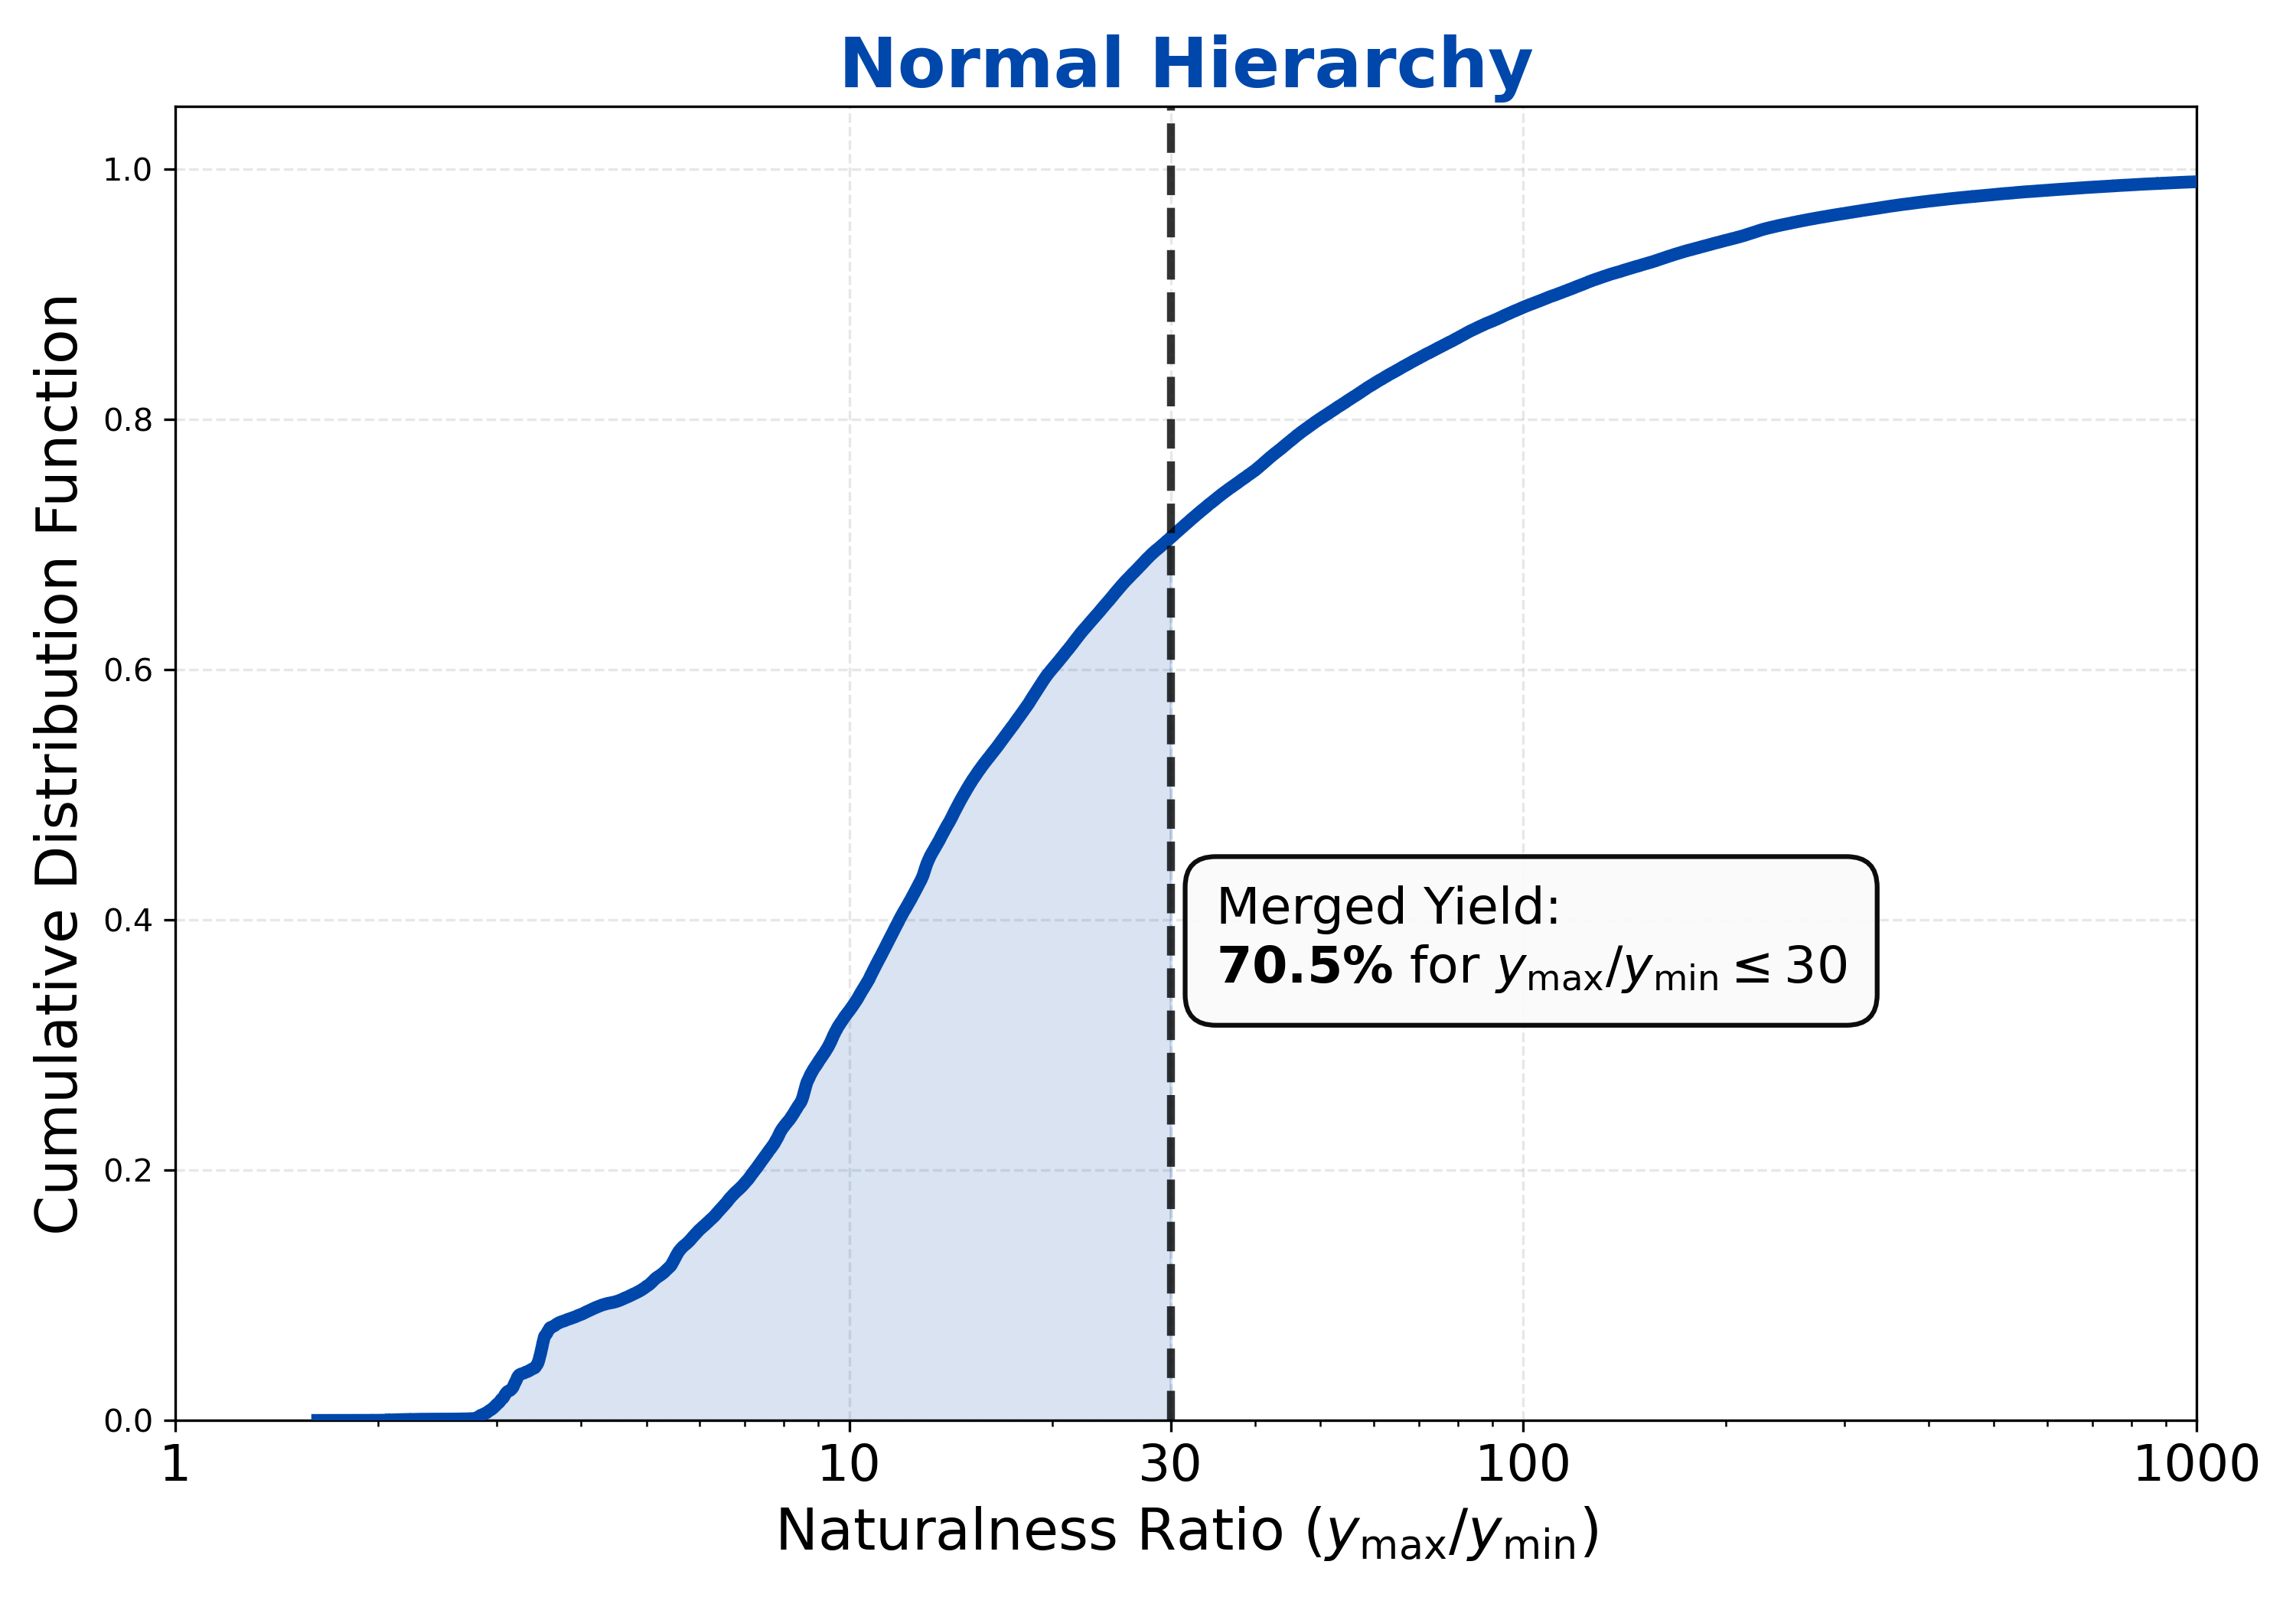
\includegraphics[width=0.7\textwidth]{../Python/Data/Normal/Merged_CDF_NH_Yukawa.png}
    \caption{Cumulative Distribution Function of the ratio $Y_{\text{max}}/Y_{\text{min}}$}
    \label{fig:Normal_spread}
\end{figure}
The posterior means of the predicted angles, heavy neutrino mass scale and the mass-squared differences are presented in \cref{fig:CornerPlot_NO_angles} and \cref{fig:CornerPlot_NO_masses}, which were generated using the Python module \texttt{corner}(v2.2.3)\cite{corner}. 
The posterior shown in $(\epsilon, \log_{10} M_0)$ plane is predominantly
connected, and concentrated near $\epsilon \sim 0.43$, as expected from our
analytical calculation \cref{eq:epsilon-estimate}. The posterior means of the
three mixing angles and the two mass squared differences are given in
\cref{tab:NO_Posteriors}, and all five observables agree with the
best fit values from \cref{tab:neutrino_angles_masses} to within
$1\sigma$.

\begin{figure}[h!]
    \centering
    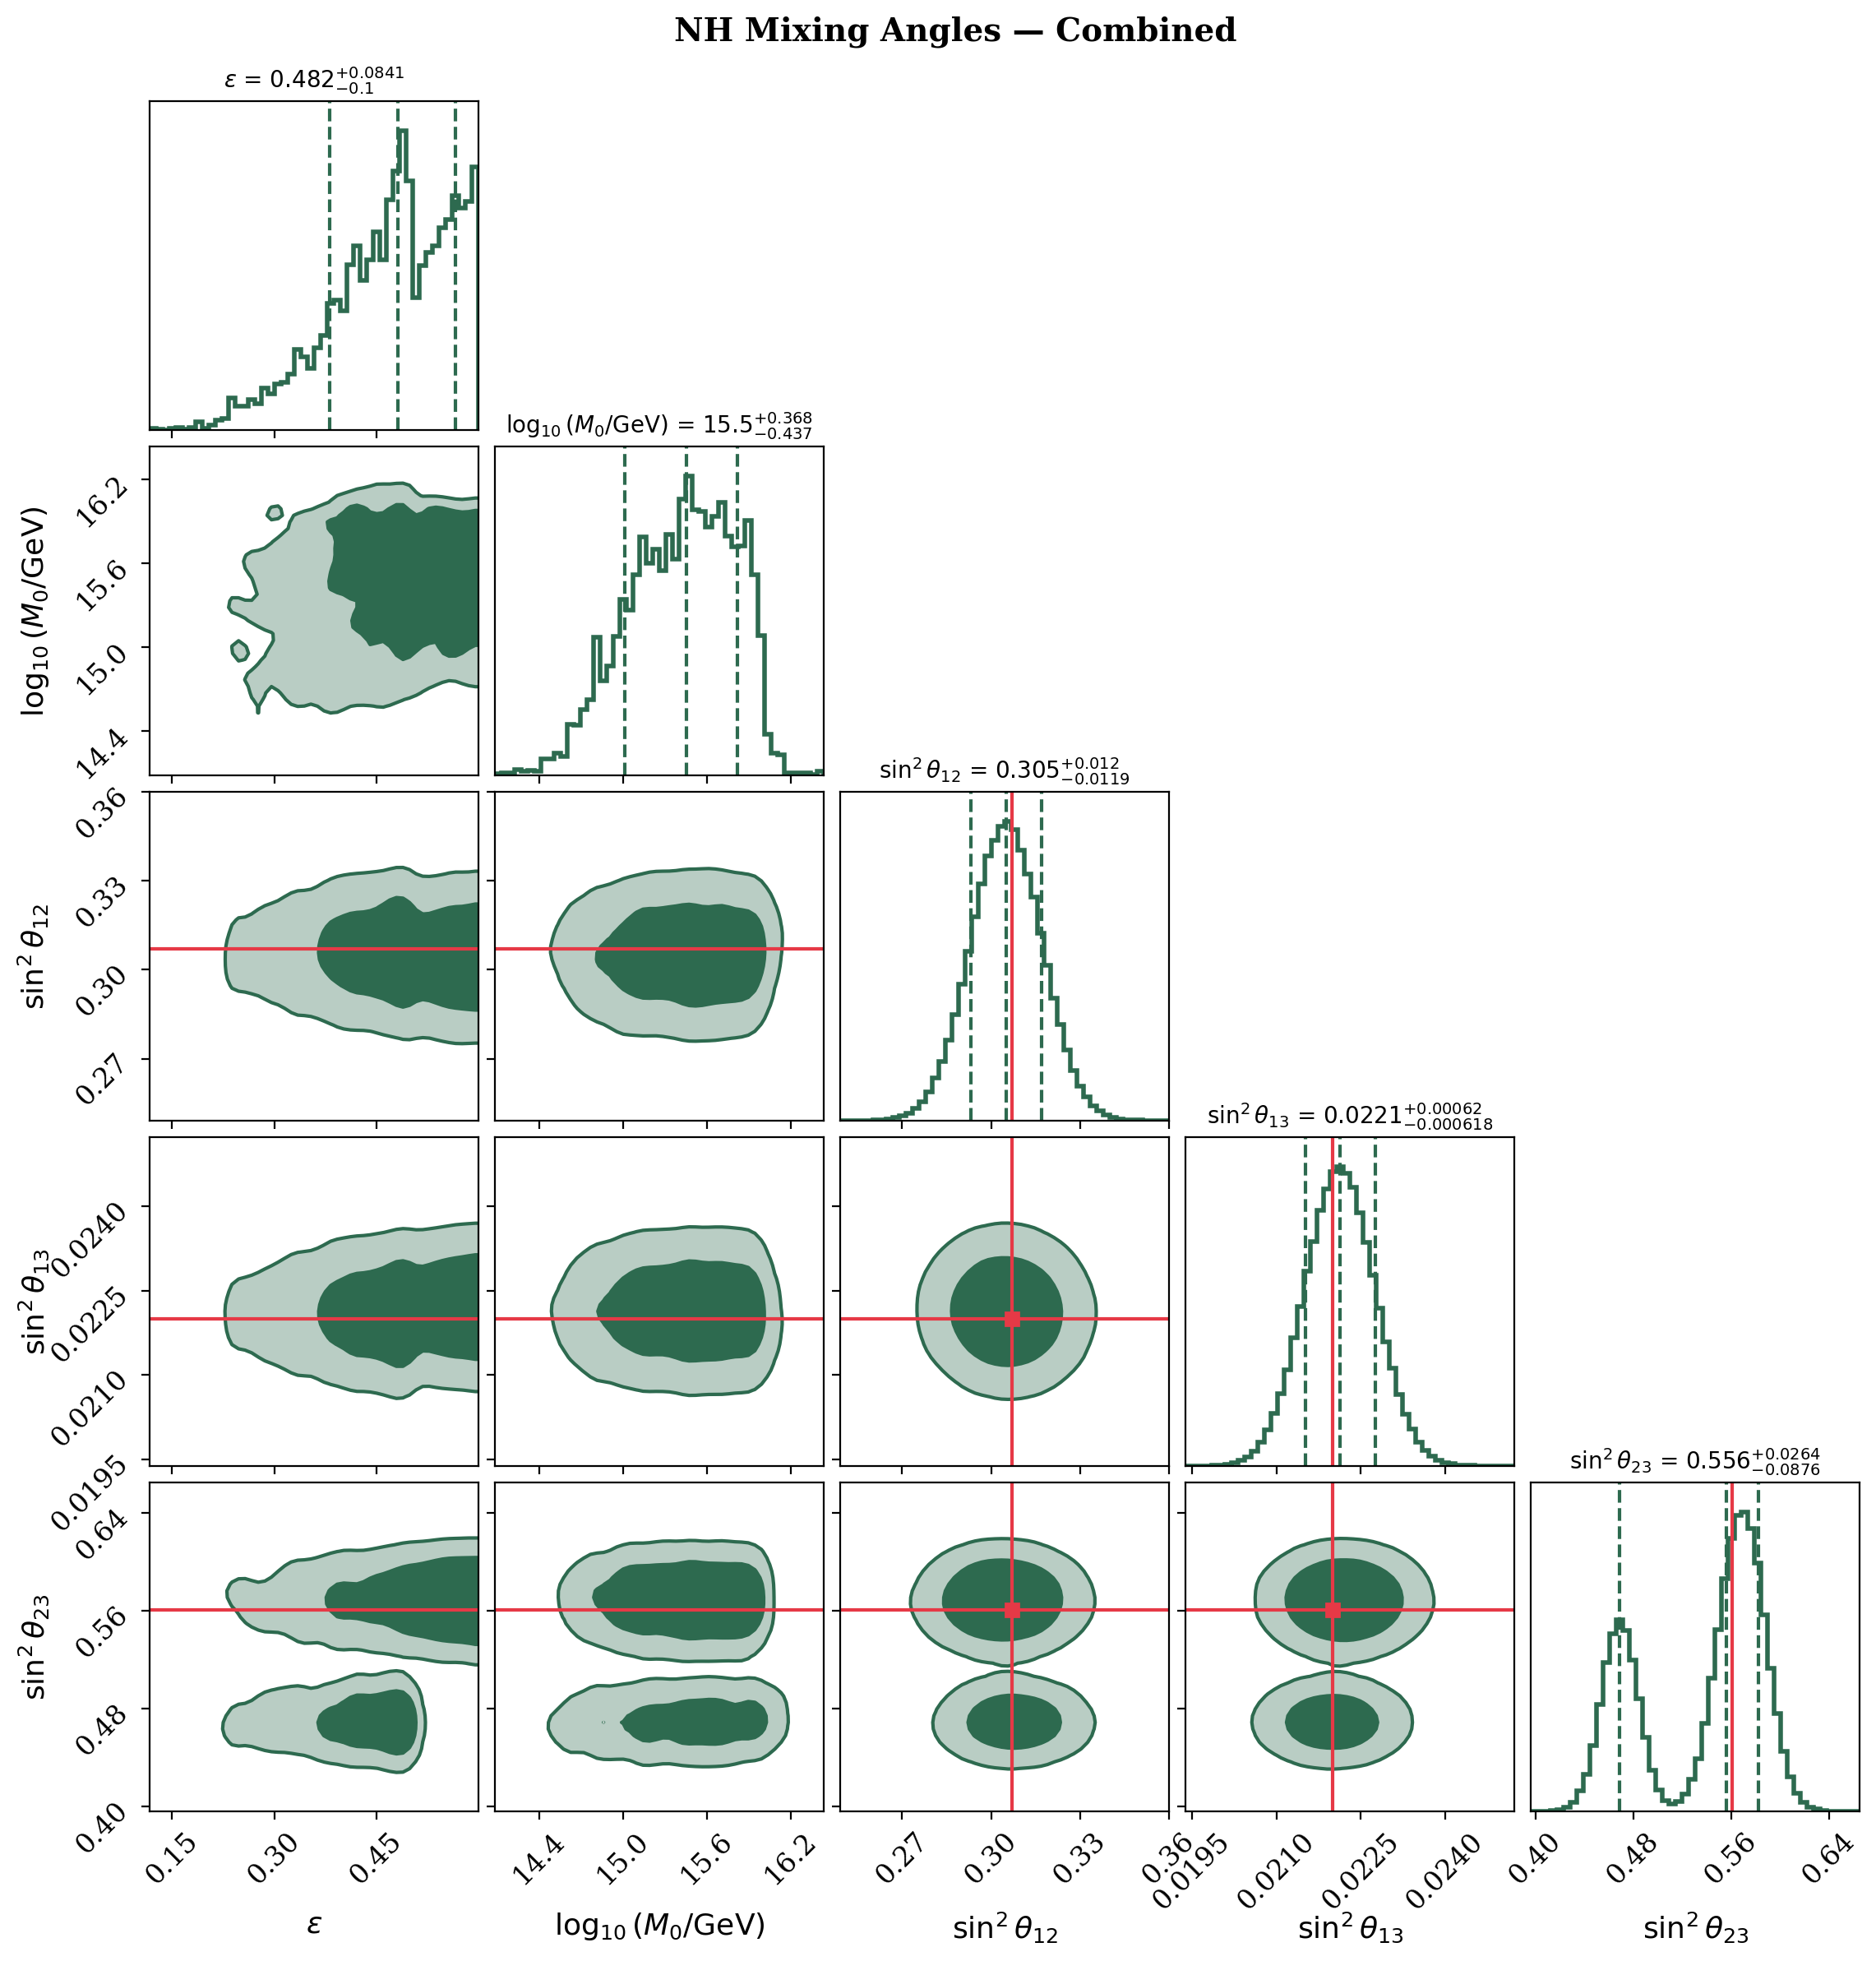
\includegraphics[width=0.9\textwidth]{../Python/Data/Normal/Corner_NH_Angles.png}
    \caption{Posterior probability distributions of the mass scale, FN parameter and the mixing angles (Normal Ordering).}
    \label{fig:CornerPlot_NO_angles}
\end{figure}
\begin{figure}[h!]
    \centering
    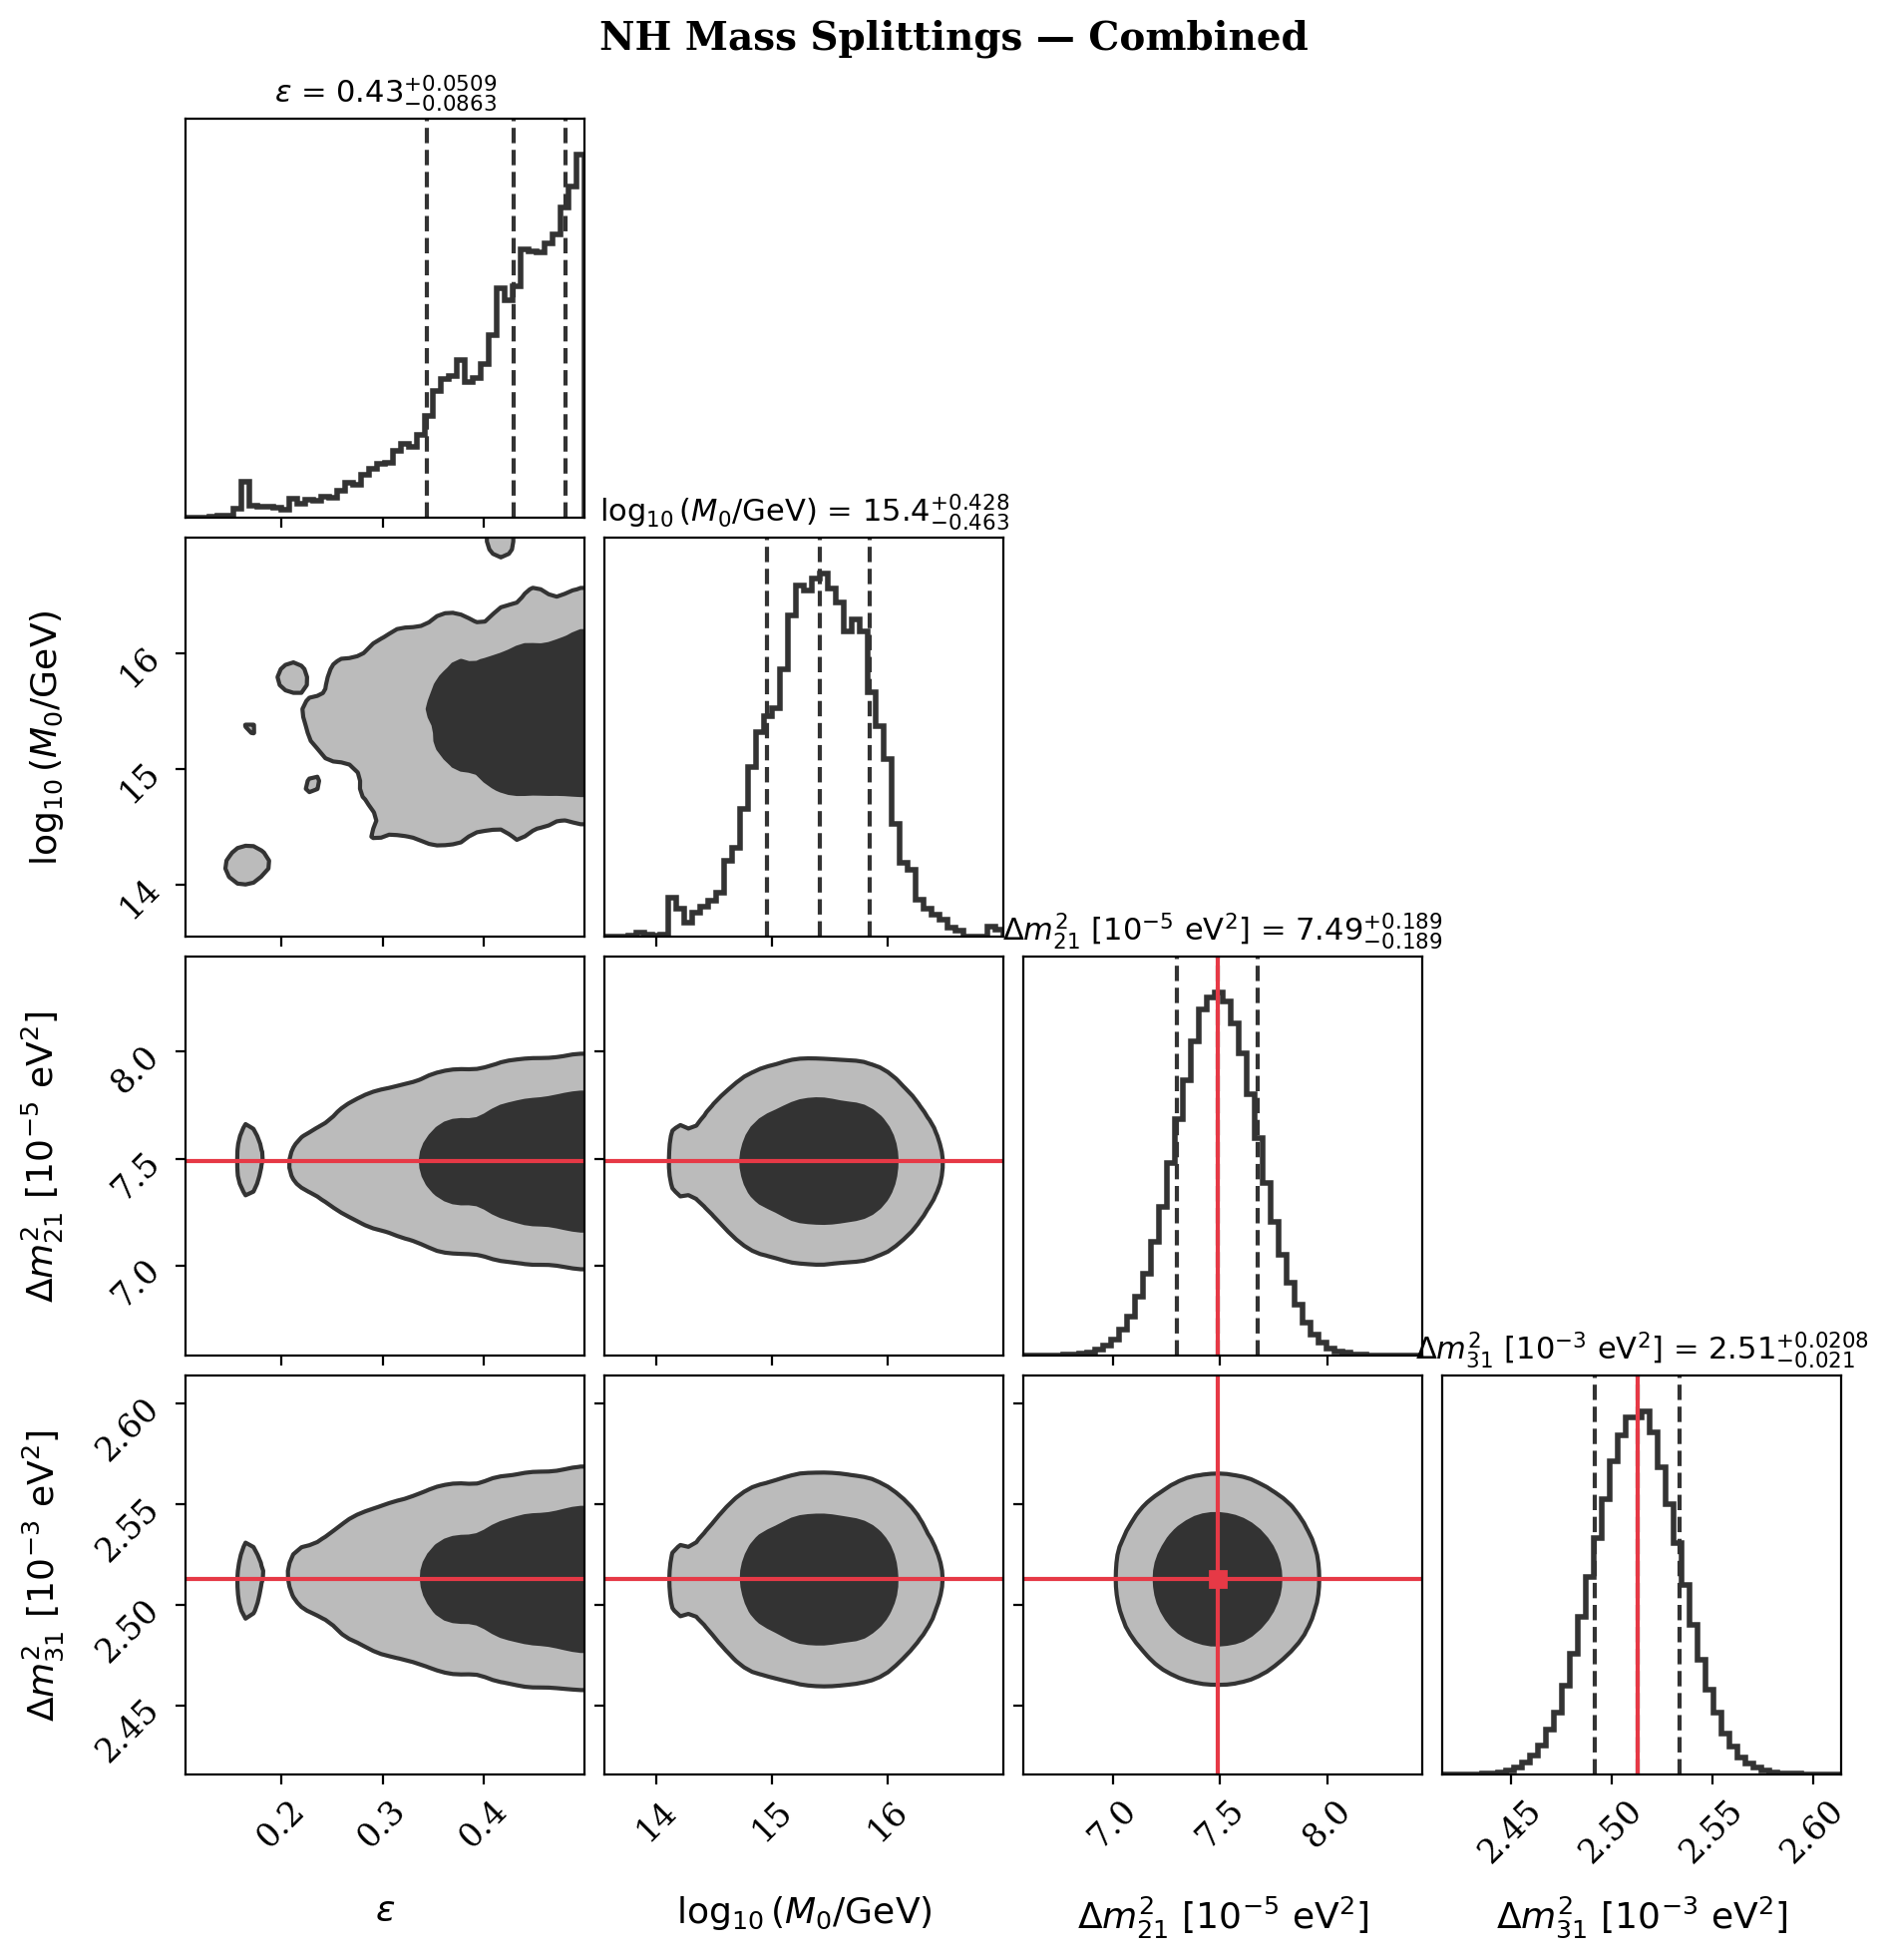
\includegraphics[width=0.9\textwidth]{../Python/Data/Normal/Corner_NH_Masses.png}
    \caption{Posterior probability distributions of the mass scale, FN parameter and the mass squared differences (Normal Ordering). The solid contours correspond to the 68$\%$ and 95$\%$ Bayesian credibility intervals.}
    \label{fig:CornerPlot_NO_masses}
\end{figure}
\begin{comment}
    \bca{Somewhere, it's worth showing the 1d distributions of delta m$^2$ parameters along with that of epsilon and of $M_0$. Also, please increase the font sizes on the graphics. You'll be showing this through a dodgy projector while giving a talk at some point and no one will be able to read them - a common, but entirely avoidable, mistake! Also, say what the vertical dashed lines mean. Also, you want to quote the mean value and standard deviations to the same number of decimal places.  } 
    
    \bca{Too many significant figures in the digits. They are distracting - superfluous information. Put uncertainties on the experimental and theoretical values. $p$-value should be $p-$value and the convention is to quote eg $.975$ rather than $0.975$ for $p-$values.}
    \bca{I suspect that $\sigma_{comb}$ makes
        no sense and should be deleted. For this, you've added the sampled and
    input standard deviations in quadrature? This makes no sense I think.}
\end{comment}

\begin{table}[h!]
    \centering
    \begin{tabular}{|c|c|c|}
      \hline
        Observable & Posterior (mean $\pm 1 \sigma$) & Experimental (mean $\pm$ 1$\sigma$) \\
        \hline
        \hline
        $\Delta m_{21}^2$/eV$^2$ & $(7.49 \pm 0.19)\times 10^{-5}$ & $(7.49 \pm 0.19)\times 10^{-5}$  \\
        $\Delta m_{31}^2$/eV$^2$ & $(2.51 \pm 0.02)\times 10^{-3}$ & $(2.51 \pm 0.02)\times 10^{-3}$ \\
        $\sin^2\theta_{12}$ & $0.3079 \pm 0.0115$ & $0.3080 \pm 0.0115$  \\
        $\sin^2\theta_{13}$ & $0.0221 \pm 0.0006$ & $0.0221 \pm 0.0006$ \\
        $\sin^2\theta_{23}$ & $0.4693 \pm 0.0149$ & $0.4700 \pm 0.0150$  \\
        \hline
    \end{tabular}
    \caption{Posterior means and 1$\sigma$ theoretical uncertainties for the Normal Ordering (NO) fit
      under Nested Sampling. The experimental values and uncertainties are
      taken from {\tt NuFIT 6.0} (2024) global fits (with SK data)
      \cite{esteban_nufit-60_2024}.}
    \label{tab:NO_Posteriors}
\end{table}
We see from \cref{tab:NO_Posteriors} that the sampled posterior means of
neutrino mass squared differences and mixing angles are all very similar to
the experimental inputs. This is no surprise since our system is
underconstrained and has more parameters than it does measured experimental
parameters.
\subsection{Inverted Hierarchy} \label{sec:Inverted Hierarchy}
Setting the Majorana matrix elements $a_{11} = a_{13} =0$,
we get an inverted
mass hierarchy. A possible way to generate this suppression is detailed in the Appendix \ref{Sec:Clockwork}.
\begin{comment}
    We have not found an effective natural way of imposing this condition using
further clockwork extensions to the model, so either some other mechanism
should be at work or the three parameters just happen to be small by chance.
\bca{Is this correct? How much suppression do we need?}
\end{comment}
%% The effective operators are obtained by integrating out the heavy
%% vector-like fermion mediators present in the UV theory, as depicted in
%% \cref{fig:spag}.  We assume the UV spectrum is incomplete and therefore lacks
%%the specific mediators required to generate these elements.
We now show that with
these texture zeroes, we obtain an inverted hierarchy:
\begin{equation} \label{eqn:IOtexture}
    M_R = M_0
    \begin{pmatrix}
    0&\epsilon^{3}a_{12}&0\\
    
    \epsilon^{3} a_{12} & \epsilon^{4} a_{22}& \epsilon^{2} a_{23}\\
    
    0 & \epsilon^{2}a_{23}&a_{33} 
    \end{pmatrix}.
\end{equation}

We once again expand the matrix $m_\nu$ as a series in $\epsilon$ after factoring out the common factors, 
\begin{equation}
    m_\nu = \frac{v^2}{2M_0} \epsilon^{-3} (X^{(0)} + \epsilon X^{(1)} + \epsilon^2 X^{(2)} + \cdots) 
\end{equation}
where 
\begin{equation}
    X^{(0)} = \begin{pmatrix}
        0 &  \times & 0 \\
        \times  & 0  &  0  \\
        0  & 0  & 0
    \end{pmatrix}, \,\,\,\,  X^{(1)} = \begin{pmatrix}
        \times & 0 & 0 \\
        0 &  \times &\times  \\
        0  & \times & 0
    \end{pmatrix}, \,\,\,\, 
     X^{(2)} = \begin{pmatrix}
    0 & \times & \times \\
    \times & 0& 0  \\
    \times& 0&0 
    \end{pmatrix}
\end{equation}
We once again collect the overall coefficient setting the mass scale $m := \frac{v^2}{2M_0}\epsilon^{-3}$ as in \cref{sec:Normal Hierarchy}, we obtain
mass eigenvalues\footnote{We fix the neutrino fields' phases here such that all masses $m_{i} \geq 0$.} (masses) 
\begin{comment}

\begin{equation} \label{eqn:Majorana_UVcompletion}
    -\mathcal{L}_{M} \supset \lambda S_{ij} \overline{\nu^c_{Ri}} \nu_{Rj} + M_{ij}^2 |S_{ij}|^2 + c_{ij} S_{ij}^\dagger \theta^{X_i + X_j} + \text{H.c.},
\end{equation}
which after $\langle \theta \rangle \neq 0$, induces the suppressed entries in the Majorana mass matrix. In this construction, the fields $S_{ij}$ are SM singlets and carry FN charges $-X_i-X_j$. To obtain the inverted hierarchy, we assume the scalar mediators $S_{11}, S_{13}$ (as depicted in \cref{eqn:Majorana_UVcompletion} and \cref{fig:Majorana_UVcompletion}) do not exist in the UV completion.
\begin{figure}[t]
    \centering
    \begin{tikzpicture}
      \begin{feynman}
        % --- Left Side Vertices ---
        % Adjusted y-coordinates slightly for better aspect ratio
        \vertex (nu_c) at (0, 3);
        \vertex (nu)   at (0, -1);
        \vertex (s_vertex) at (2, 1);

        % --- Central Blob ---
        \node[blob, minimum size=0.8cm] (blob_vertex) at (5, 1) {};

        % --- Right Side Vertices
        \vertex (theta_top) at (9, 3.5) {\(\langle \theta \rangle\)};
        \vertex (theta_1) at (8.8, 2.25);
        
        \vertex (theta_mid) at (9.2, 1) {\(\langle \theta \rangle\)};

        \vertex (theta_2) at (8.8, -0.25);
        
        \vertex (theta_bot) at (9, -1.5) {\(\langle \theta \rangle\)};

        % --- Diagram Connections ---
        \diagram*{
          % Left side (unchanged)
          (nu_c) --[anti fermion, edge label'={\(\overline{\nu^c_{Ri}}\)}] (s_vertex),
          (nu)   --[fermion, edge label'={\(\nu_{Rj}\)}] (s_vertex),
          (s_vertex) --[scalar, edge label={\(S_{ij}\)}] (blob_vertex),

          % Right side: Connect blob to representative flavons
          (blob_vertex) -- [scalar] (theta_top),
          (blob_vertex) -- [scalar] (theta_mid),
          (blob_vertex) -- [scalar] (theta_bot),

            (blob_vertex) -- [scalar] (theta_1),
          (blob_vertex) -- [scalar] (theta_2),

        };
      \end{feynman}

      % --- Post-Diagram Annotations ---

      % 1. Add floating visual dots BETWEEN the lines to suggest continuity.
      % We use the 'calc' library syntax ($(A)!0.5!(B)$) to find midpoints.
      \node at ($(blob_vertex)!0.6!(theta_top) + (1.5,-0.5)$) {$\vdots$};
      \node at ($(blob_vertex)!0.6!(theta_bot) + (1.5, 0.5)$) {$\vdots$};

      % 2. Add the Curly Brace Label
      % This draws a brace from the top theta to the bottom theta on the right side.
      \draw[decorate, decoration={brace, amplitude=10pt}, thick]
           ($(theta_top.north east)+(0.1,0)$) -- ($(theta_bot.south east)+(0.1,0)$)
           node [midway, right=15pt, align=center, font=\small] {\(X_i + X_j\) \\ insertions};

    \end{tikzpicture}
    \caption{The Feynman diagram showing the generation of the effective Majorana mass operator $A\left(\frac{\langle\theta \rangle}{\Lambda_{\text{FN}}} \right)^{X_i+X_j} \overline{\nu_{Ri}^c}  \nu_{Rj}$. The intermediate heavy scalar $S_{ij}$ couples to the flavon field $\theta$ through an effective vertex (represented by the blob), requiring $X_i+X_j$ insertions of the VEV to maintain gauge invariance, resulting in the suppression factor $(\langle\theta \rangle/\Lambda_{\text{FN}})^{X_i+X_j}$.}
    \label{fig:Majorana_UVcompletion}
\end{figure}

    \bca{I presume that we should do a field phase redefinition to change an overall minus in $m_2$ here - it'll make it much clearer.}
    
    see \cref{fig:spag}) \bca{Detail the field content of the UV model here.} for these specific entries, hence forbidding them
    
    \bca{Note that one uses $\sim$ usually for order of magnitude estimates or "goes like" arguments, or $\approx$ for an approximation. SHould these symbols change in the following?}
    \left( \frac{7.5 \times 10^{-5}}{
      2.5 \times 10^{-3}} \right)
\end{comment}
\begin{align}
    m_1 &= m \left(A + \epsilon B + \epsilon^2 C+{\mathcal{O}}(\epsilon^3) \right)\\
    m_2 &= m \left(A - \epsilon B+  \epsilon^2 C+{\mathcal{O}}(\epsilon^3) \right)\\
    m_3 &= m{\mathcal{O}}(\epsilon^3),
\end{align}
i.e.\ an inverted hierarchy (i.e.\ $m_3 \ll m_1 < m_2$) where
\begin{align}   
    \frac{\Delta m_{21}^2}{|\Delta m_{32}^2|} &\approx \frac{4m^2AB \epsilon}{m^2 A^2} \Rightarrow
    0.03 \approx 4 \Big(\frac{B}{A}\Big)\epsilon \quad\Rightarrow\quad
    \epsilon \sim \mathcal{O}(1) \times0.03,\label{ep}
\end{align}
The PMNS matrix has the (unnormalized) form,
\begin{equation}
    U =
    \begin{pmatrix}
        -1+ \epsilon u_{11}^{(1)} +\epsilon^2 u_{11}^{(2)} & 1 + \epsilon u_{12}^{(1)} +\epsilon^2 u_{12}^{(2)} & \epsilon u_{13}^{(1)} +\epsilon^2 u_{13}^{(2)} \\
        1 + \epsilon u_{21}^{(1)} +\epsilon^2 u_{21}^{(2)} & -1 + \epsilon u_{22}^{(1)} +\epsilon^2 u_{22}^{(2)} &  \epsilon u_{23}^{(1)} +\epsilon^2 u_{23}^{(2)} \\
        -\epsilon u_{31}^{(1)} &  \epsilon^2 u_{32}^{(2)} & 1 + \epsilon^2
        u_{33}^{(2)}
    \end{pmatrix} + {\mathcal O}(\epsilon^3),
\end{equation}
giving us the mixing angles, 
\begin{align}
    \sin \theta_{13} &= |U_{e3}| \approx  \epsilon u_{13}' +\epsilon^2 u_{13}'' \\
    \tan \theta_{12} &= \frac{|{U_{e2}}|}{{|U_{e1}|}} \approx \frac{1 + \epsilon u_{12}' +\epsilon^2 u_{12}''}{-1 + \epsilon u_{11}' +\epsilon^2 u_{11}''}\approx 1 + \epsilon u_{12}' +\epsilon^2 (u_{12}'' - u_{11}') \\
    \tan \theta_{23} &= \frac{{|U_{\mu3}|}}{|{U_{\tau3}}|} \approx \frac{ \epsilon u_{23}' +\epsilon^2 u_{23}''}{ 1 +\epsilon^2 u_{33}''}.
\end{align}
We have therefore shown again that if the $u_{ij}^{(k)}$ parameters are of order 1 and $\epsilon \sim 0.03$, then we can fit these approximations to the data, as given in \cref{tab:neutrino_angles_masses}. This is only a leading-order analytical estimate intended to demonstrate the inverted hierarchy model's viability. 

We once again perform a global Bayesian parameter inference to map the parameter space that reproduces the observed mixing angles as in \cref{tab:neutrino_angles_masses}, using the same Python
module and configurations (\texttt{UltraNest}, $N_{\mathrm{live}} = 50000$). 
We use the same priors as in the normal ordered case, i.e.\ uniform priors
${\mathcal U}$ on all parameters. For the Frogatt-Nielson expansion parameter $\epsilon$, we once again assign a uniform prior $\epsilon \sim \mathcal{U}[0.1,0.5]$, based on our analytical arguments in \cref{ep}. The majorana mass scale is once again assigned a Jeffreys' prior, such that the prior distribution of it's logarithm is uniform, $\log_{10} M_0 \sim \mathcal{U}[13,17]$. The rest of the Yukawa and Majorana elements are assigned uniform priors, $\mathcal{U}[-3,3]$ similarly.

\begin{comment}
$\epsilon \sim
\mathcal{U}[0.1,0.5], \,\ \log_{10}M_0 \sim \mathcal{U}[13.0,17.0], \,\ y_{ij}
\sim \mathcal{U}[-3,3] \,\ \text{and} \,\ a_{ij} \sim \mathcal{U}[-3,3]$.
\bca{This is confusing. (\ref{ep}) states that we fix $\epsilon$ to a definite
  value, but here we say we vary it. Which is it?}

\end{comment}

We again measure the spread of the final posterior samples of the elements of the Yukawa matrix using the ratio $r = |Y_{\text{max}}|/|Y_{\text{min}}|$, this time comparing the absolute values of all nine elements. This gives,
\begin{equation} \label{IO:CDFPercent}
    P(r<30) = 69 \pm 5 \%
\end{equation}
with the standard deviation again arising from the run-to-run variance. The sampling algorithm is finding the posterior in the inverted hierarchy case much harder to converge and hence is the reason for the relatively higher variance.

\begin{comment}
    The posterior means of the predicted angles, heavy neutrino mass scale and the mass-
squared differences are presented in \cref{fig:CornerPlot_IO_angles} and \cref{fig:CornerPlot_IO_masses}, which were generated using the Python
module corner(v2.2.3)\cite{corner}.

\end{comment}

The physics observables, however, such as the
three mixing angles and the mass-squared differences, all converge to the
NuFIT-6.0 \cite{esteban_nufit-60_2024} best fit values within $1 \sigma$. This
is presented in \cref{tab:IO_Posteriors} and in the corner plots \cref{fig:CornerPlot_IO_angles} and \cref{fig:CornerPlot_IO_masses}. Given the CDF percentage
uncertainties, we can say that in the \model, both mass orderings (Normal
ordering or Inverted ordering) are statistically similar, with approximately
$2/3$ of the posterior volume in both cases being satisfying $r<30$, which one
could argue is natural.

\begin{comment}

This
larger uncertainty relative to the normal-ordering case \cref{NO:CDFPercent}
is due to the more difficult, disconnected posterior topology of the Inverted
ordering. \bca{I see scant evidence of this! Suggest instead: The sampling
  algorithm is finding the posterior more difficult to converge on in the
  inverted hierarchy case.}

 \bca{Prabhoda I want to talk to you about the way these fits are done: one
   could have done them a frequentist way I think, which mightn't have had the
 scanning difficulties you've encountered.}
 
While the algorithm identifies valid regions successfully, the global integration reveals a highly disjointed likelihood surface. 


While the algorithm isolates certain regions of the parameter space that appear to be highly natural, with $75.3\%$ of the samples found in the sampling run (with $10^5$ live points and $\sim 10^6$ samples), which achieved the highest Bayesian evidence ($\log Z = -29.1$), to have $r<30$.

Lower evidence runs exhibit signs of getting trapped in difficult geometry, with one having a bimodal posterior distribution in $\theta_{12}$ and a highly suppressed naturalness percentage ($\sim 65\%$). The optimal run, presented here, reveals that the true parameter volume is highly natural ($\sim 75\%$), though highly disjointed.

The corner plot generated with this data, \cref{fig:CornerPlot_IO_angles} and \cref{fig:CornerPlot_IO_masses}, reflects this analysis, showing a fragmented parameter space in the $\epsilon$ versus $\log_{10}(M_0)$ plane. Instead of a continuous plot, the posterior resolves into discrete, isolated 'islands' of high probability.
\end{comment}

\pcs{CHANGE GRAPH NAME!}

\begin{figure}[h!]
    \centering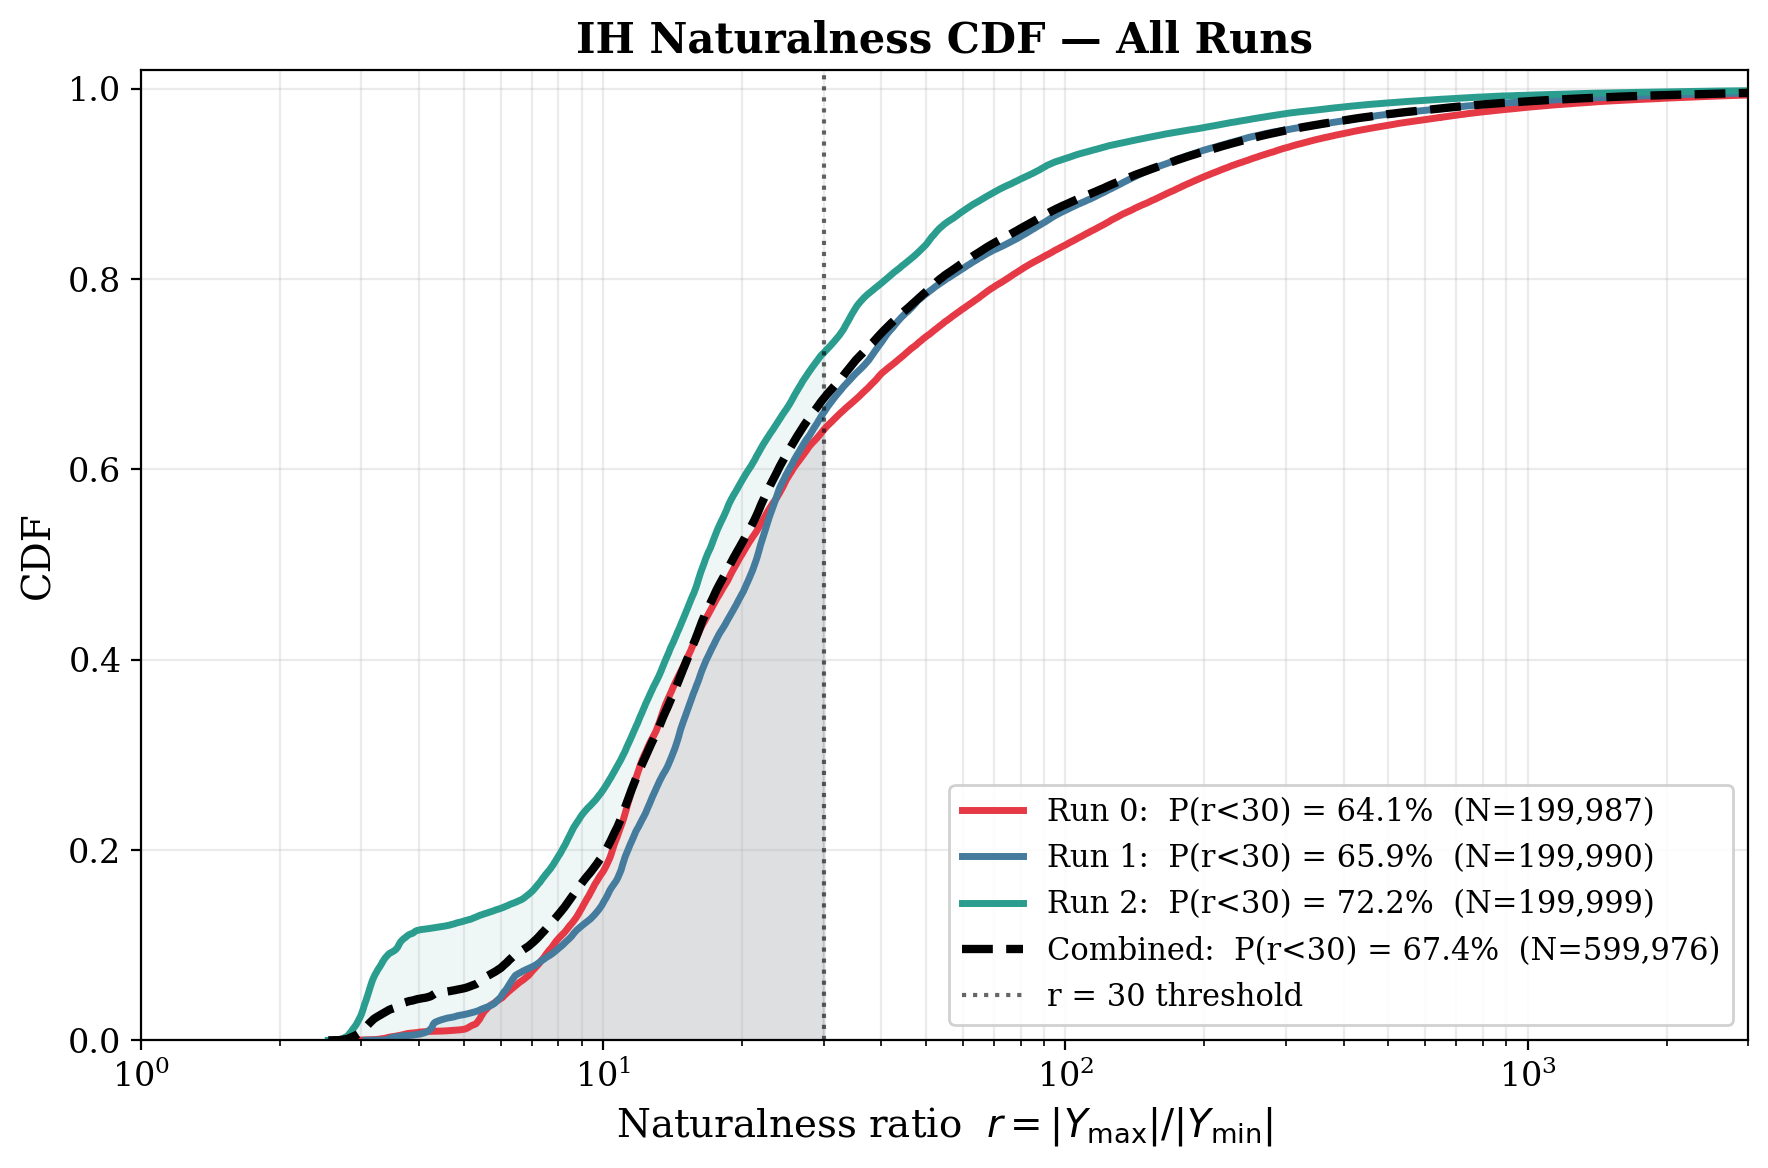
\includegraphics[width=0.7\textwidth]{../Python/Data/Inverted/Merged_CDF_IH_Yukawa.png}
    \caption{Cumulative Distribution Function of the ratio $Y_{\text{max}}/Y_{\text{min}}$}
    \label{fig:Inverted_spread}
\end{figure}
\begin{comment}
    \bca{Should all be quoted like I've done the top equation. You can ask me why next time we speak.}

    \bca{I don't see where you've put these. They need to be specified and referred to explicitly. (one may ask before what?)}
\end{comment}
\begin{figure}[h!]
    \centering
    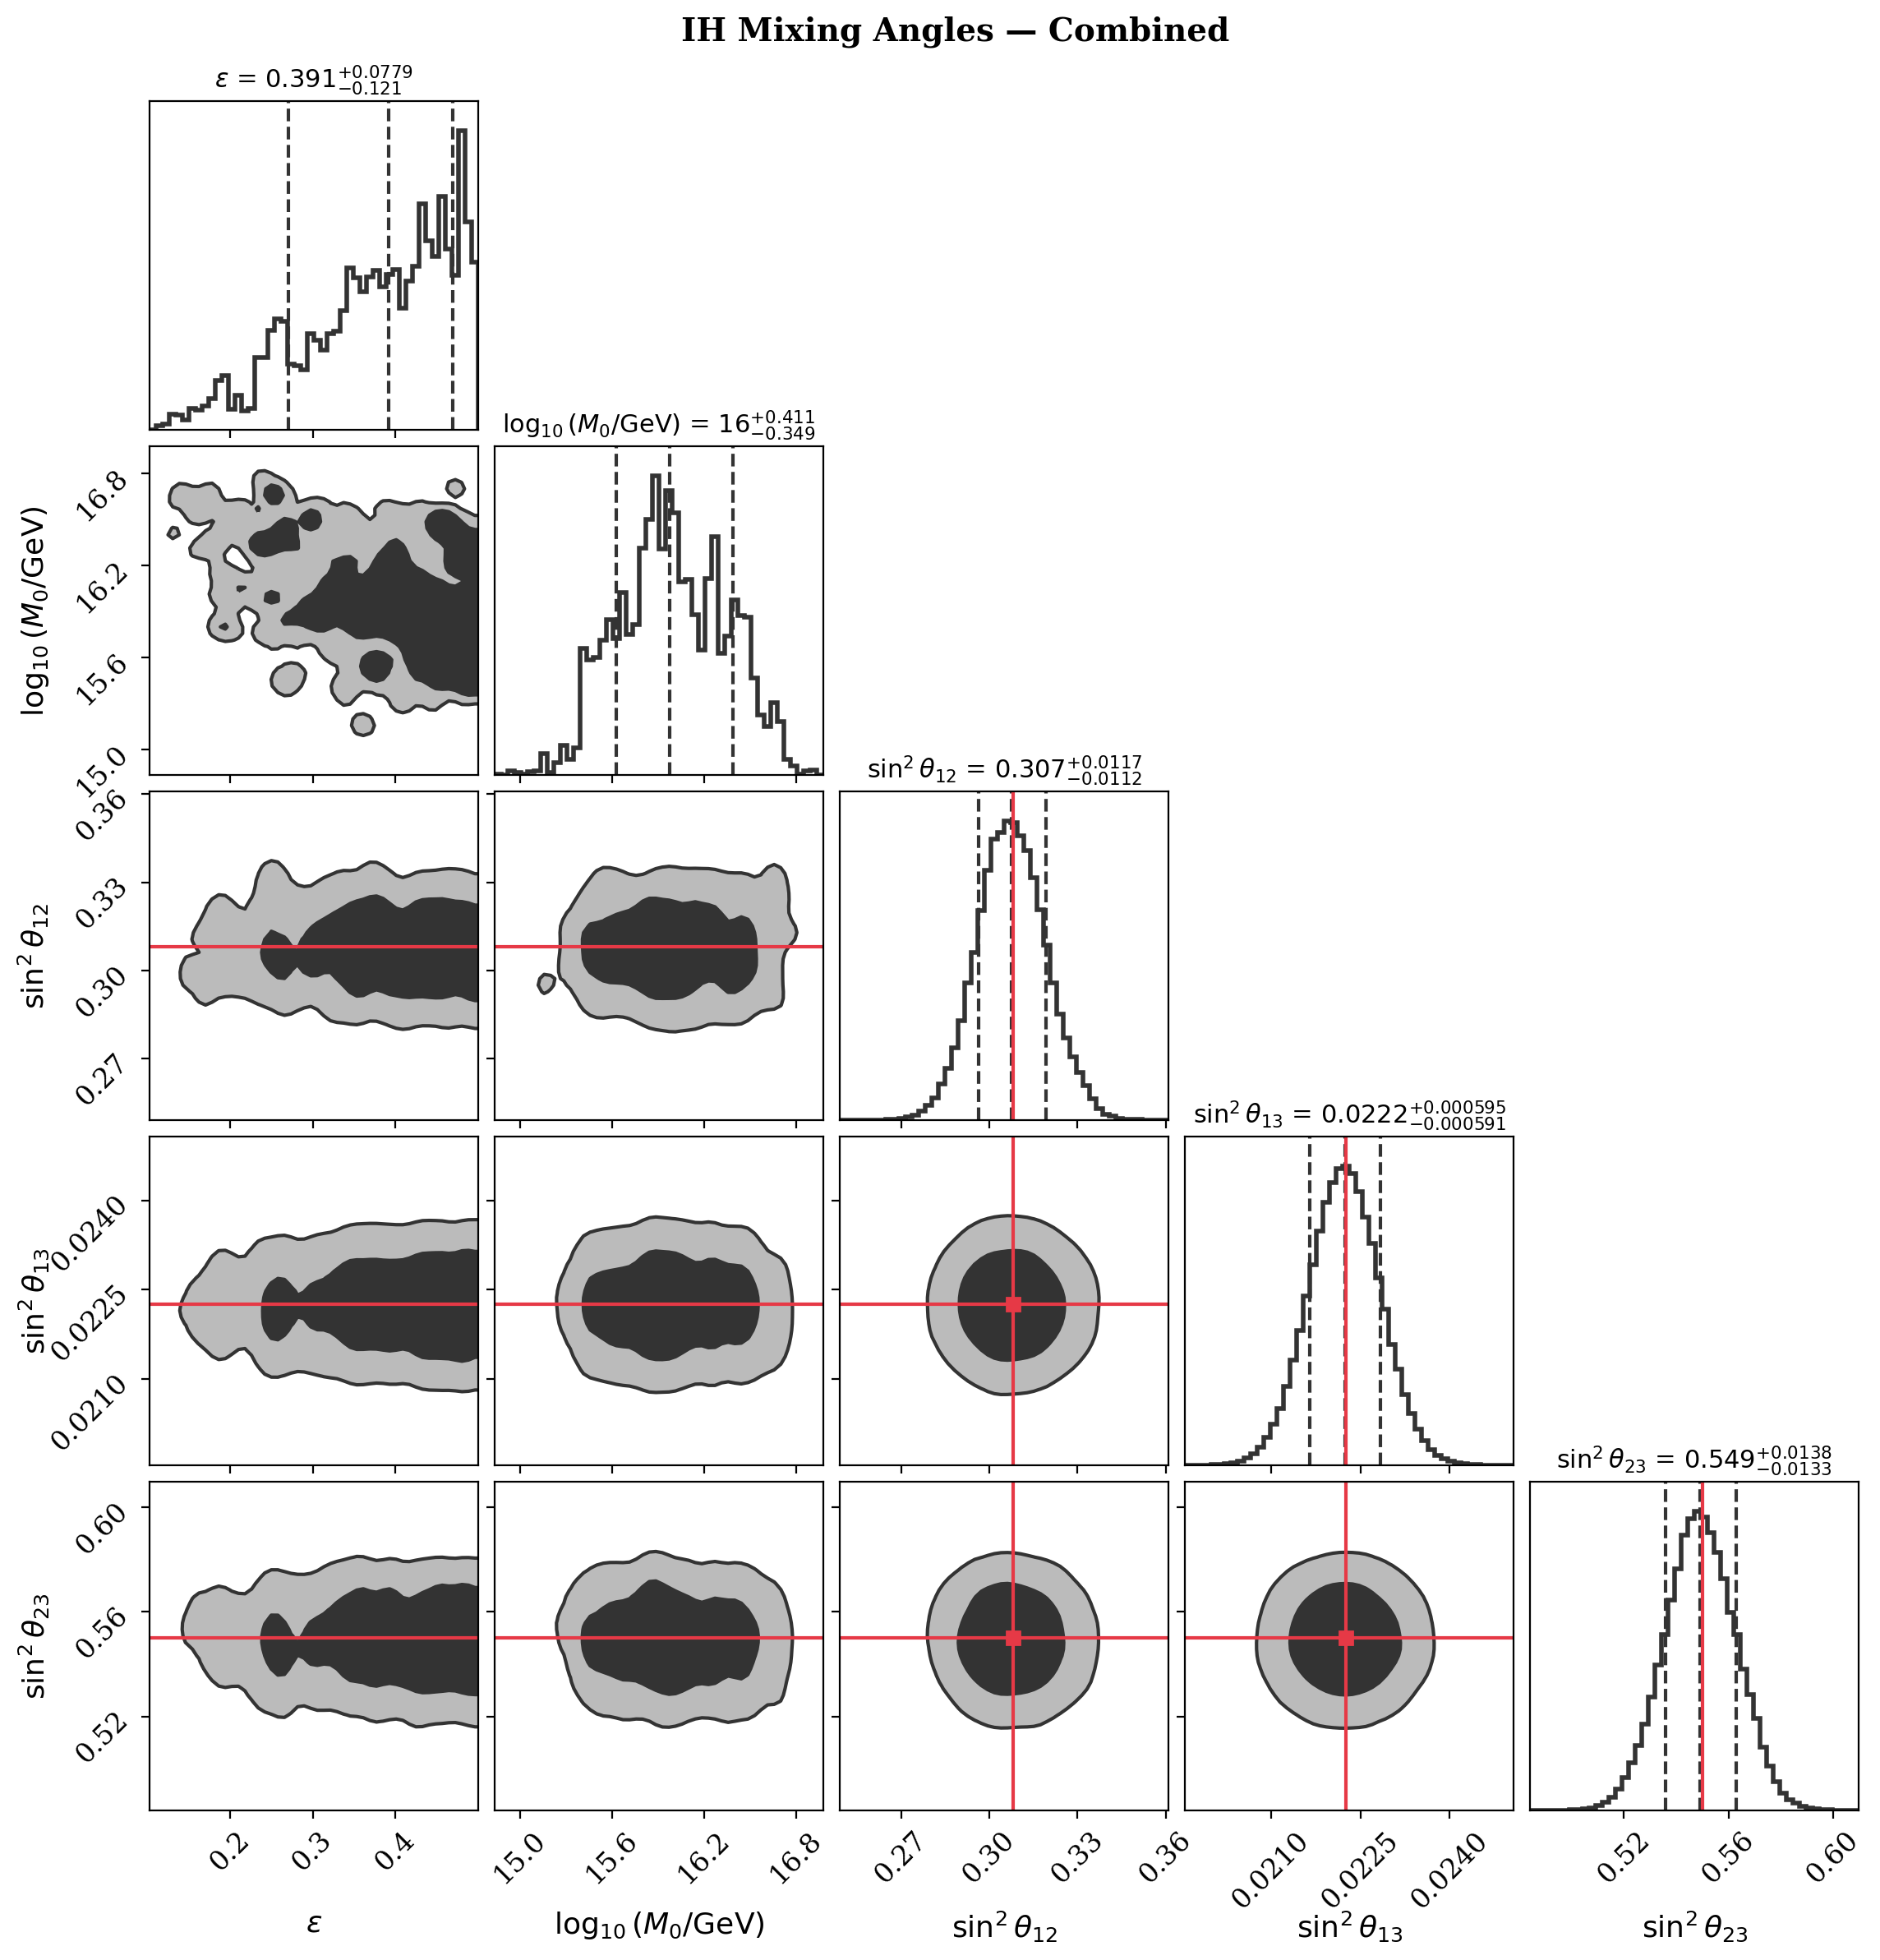
\includegraphics[width=0.9\textwidth]{../Python/Data/Inverted/Corner_IH_Angles.png}
    \caption{Posterior probability distributions of the mass scale, FN parameter and the mixing angles (Inverted Ordering).}
    \label{fig:CornerPlot_IO_angles}
\end{figure}
\begin{figure}[h!]
\centering
    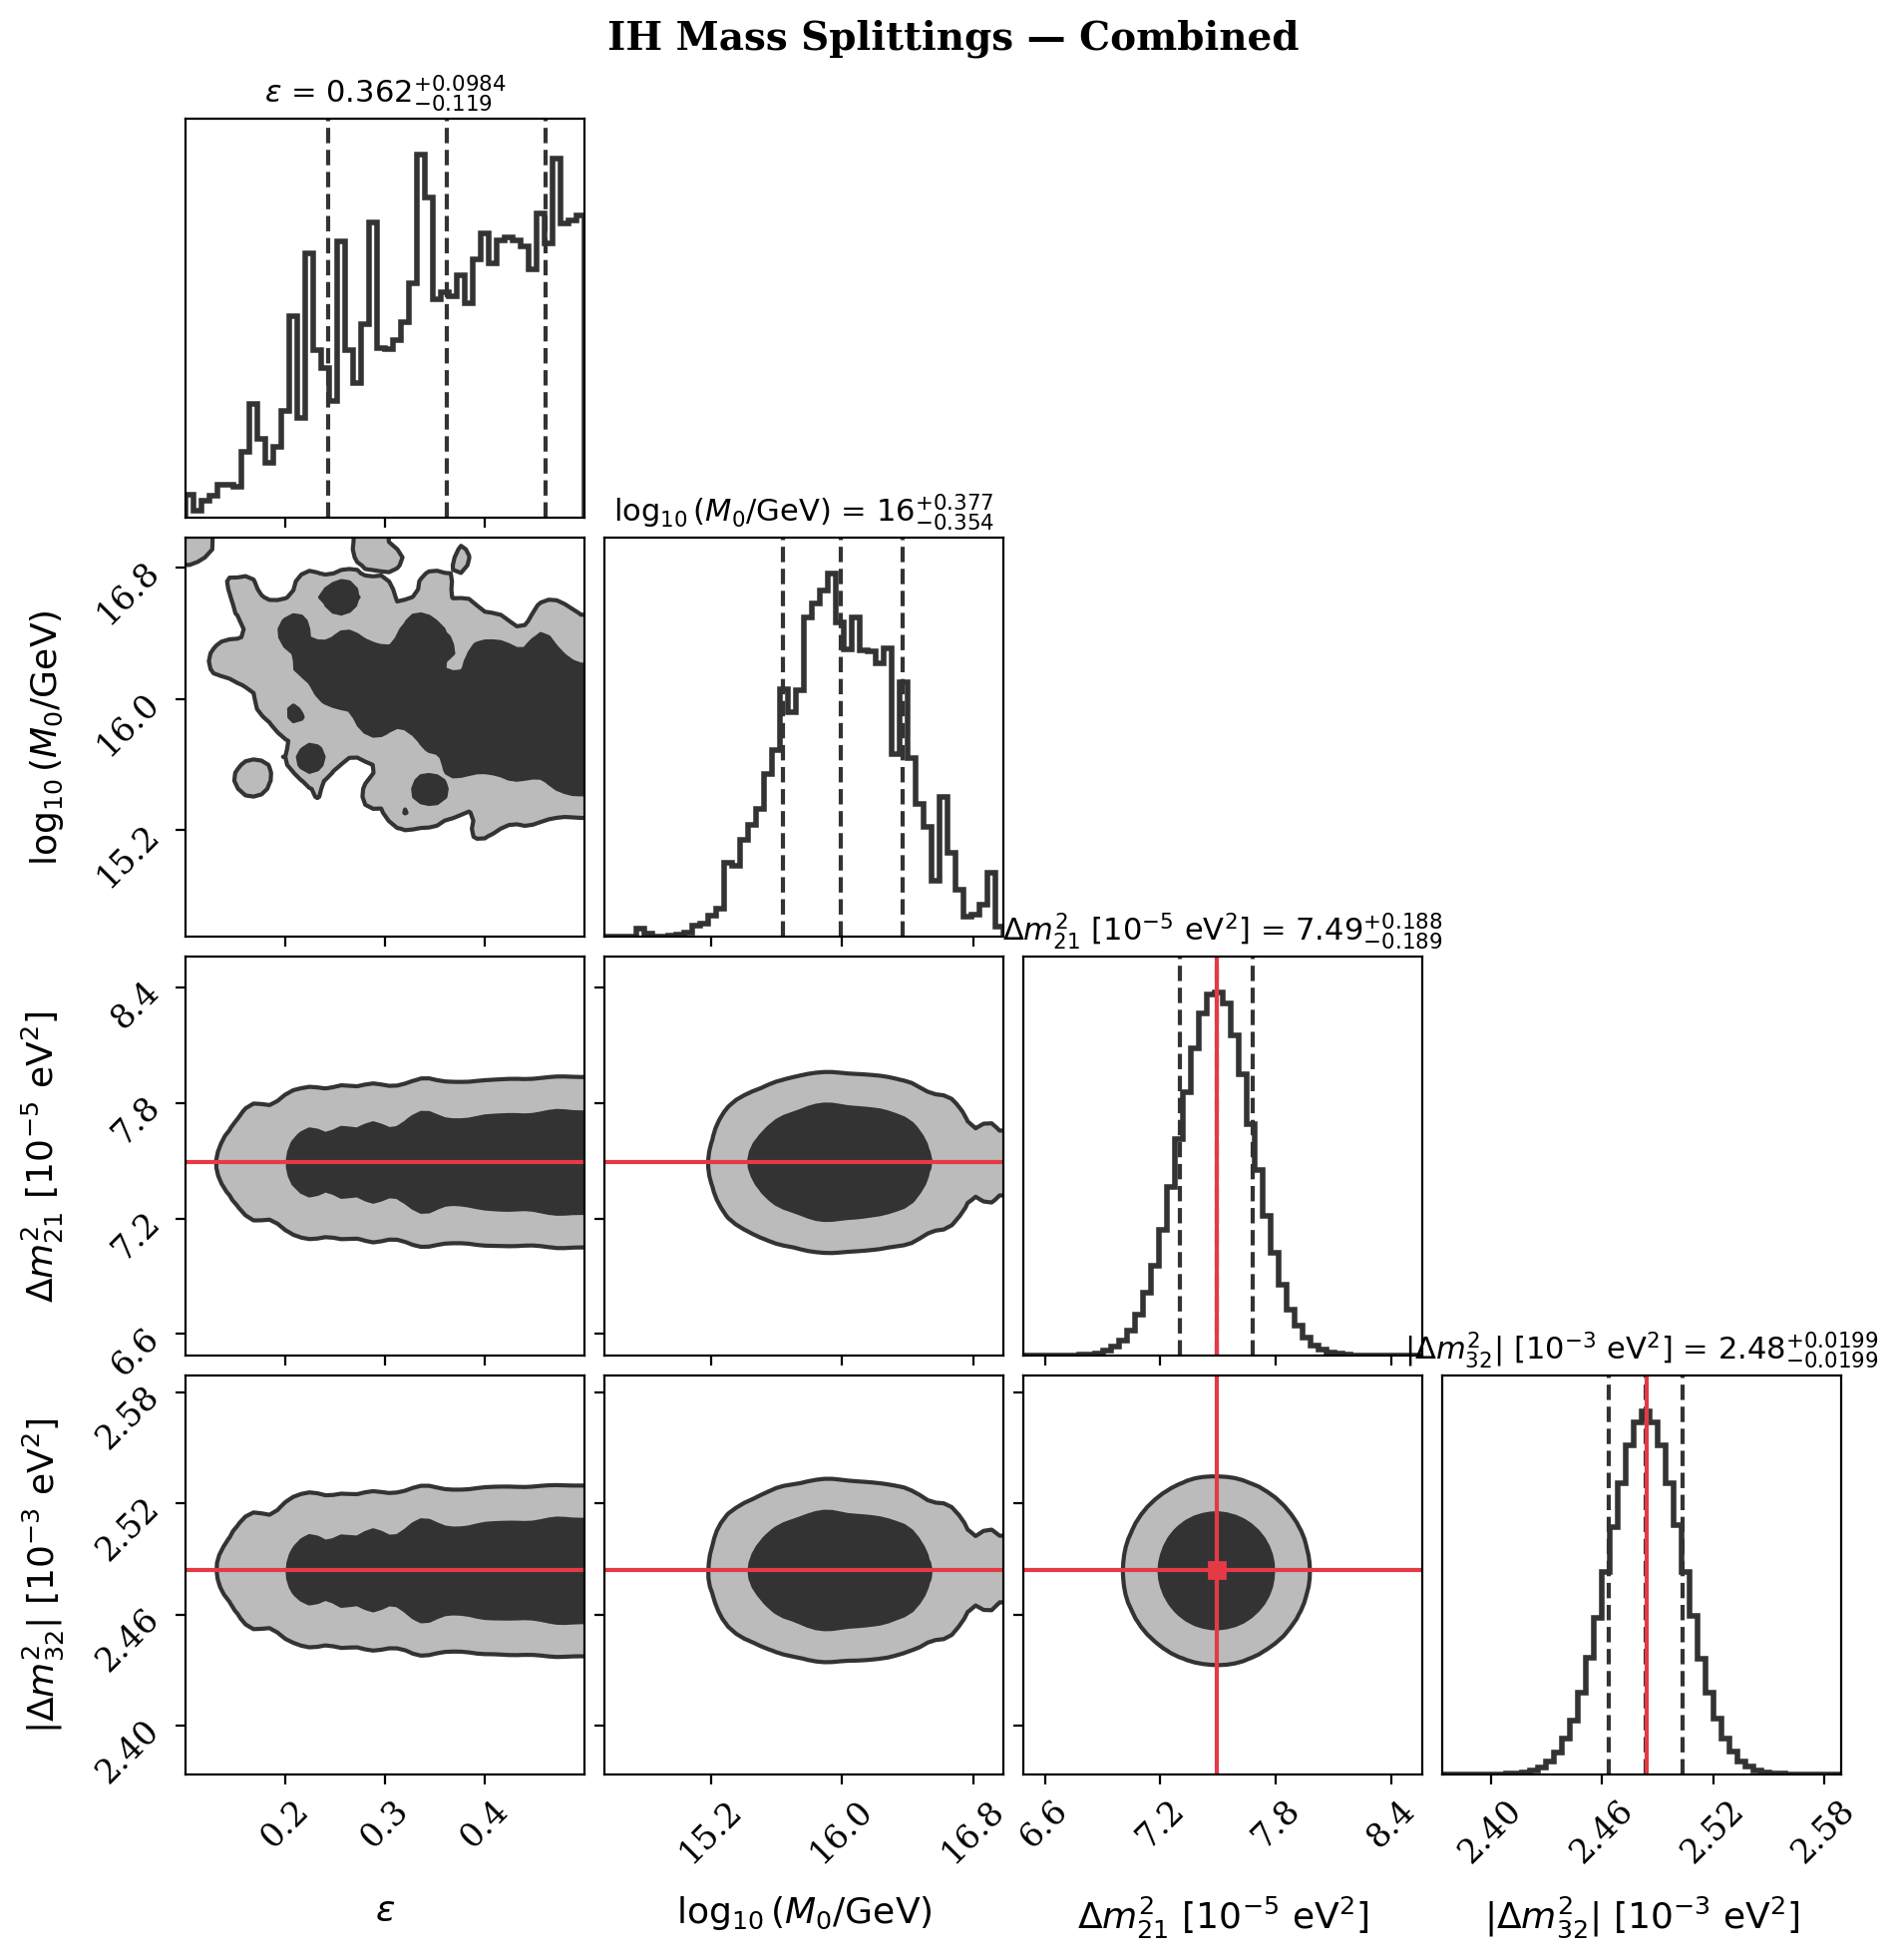
\includegraphics[width=0.9\textwidth]{../Python/Data/Inverted/Corner_IH_Masses.png}
    \caption{Posterior probability distributions of the mass scale, FN parameter and the mass squared differences (Inverted Ordering).}
    \label{fig:CornerPlot_IO_masses}
\end{figure}

\begin{table}[h!]
    \centering
    \begin{tabular}{|c|c|c|}
      \hline
        Observable & Samples (mean $\pm$ 1$\sigma$) & Experimental (mean $\pm$ 1$\sigma$) \\
        \hline
        \hline
        $\Delta m_{21}^2$ & $(7.49 \pm 0.19)\times 10^{-5}$ & $(7.49 \pm 0.19)\times 10^{-5}$  \\
        $\Delta m_{31}^2$ & $(2.48 \pm 0.02)\times 10^{-3}$ & $(2.48 \pm 0.02)\times 10^{-3}$  \\
        $\sin^2\theta_{12}$ & $0.3081 \pm 0.0114$ & $0.3080 \pm 0.0115$ \\
        $\sin^2\theta_{13}$ & $0.0222 \pm 0.0006$ & $0.0223 \pm 0.0006$ \\
        $\sin^2\theta_{23}$ & $0.5497 \pm 0.0134$ & $0.5500 \pm 0.0135$ \\
        \hline
    \end{tabular}
    \caption{Posterior means and 1$\sigma$ theoretical uncertainties for the Inverted Ordering (IO)
      fit under Nested Sampling. The experimental values and uncertainties are
      taken from {\tt NuFIT 6.0} (2024) global fits (with SK data) \cite{esteban_nufit-60_2024}.}
    \label{tab:IO_Posteriors}
\end{table}

\begin{comment}
\bca{Define SK -
      what is it?} 
    $\epsilon$ & $0.36 \pm 0.099$ &  &  &  \\
        $\log_{10} M_0$ & $15.12 \pm 0.55$ &  &  &  \\
      \hline
\end{comment}
\section{Conclusions}\label{sec:conc}
We have shown that the \model\ helps explain the small neutrino masses and sizeable leptonic mixing angles that agree with those inferred from measurements of neutrino oscillation phenomena. 
The $U(1)_X$ gauge symmetry in the \model\ is then successfully and
simultaneously put to three uses: to explain measurements involving the $b \rightarrow s l^+ l^-$ transition, to explain some of the hierarchies in neutrino masses and mixing angles and to suppress CLFV. 
A normal hierarchy in the sub-eV neutrino spectrum which agrees with oscillation measurements can be explained with all fundamental Yukawa couplings of order one except for a single coupling, which must be at the percent level. This percent-level suppression cannot be easily explained by our realisation of the FN mechanism but could be explained by other means, for example by adding a further sector of global $U(1)$ symmetries and clockwork fields, as exemplified in Appendix~\ref{Sec:Clockwork}. 
An inverted neutrino spectrum instead requires the further suppression of two fundamental Yukawa couplings beyond that implied by the FN mechanism, which again can be accomadated for in an extended clockwork mechanism model as demonstrated in Appendix~\ref{Sec:Clockwork}.

It is clear that the \model\ would need additional model building in order to further the FN proposal to fully explain all of the observed patterns in the charged fermionic fields' masses and mixing angles in detail. One requires an extra symmetry that will enforce an approximate $U(2)_q \times U(2)_u \times U(2)_R$ approximate global symmetry and make the upper left-hand block of $Y_{U,D}$ (\ref{chferms}) zero, at the level of the renormalisable terms in the Lagrangian density.
We envisage this to follow the flavour deconstruction programme~\cite{Bordone:2017bld,Greljo:2024ovt}, where the details of the lighter charged fermion masses and mixing angles will be explained further into the ultra-violet r\'egime than the multi-TeV scales headed herewith further family gauge symmetries. 


Flavour deconstruction has recently attracted attention as regards neutrino masses in other settings: since neutrino masses and mixing angles look somewhat anarchic compared to the charged fermions of the SM, it was not \emph{a priori} obvious that it would explain the patterns inferred from neutrino oscillation measurements. However, some generalities were considered in Ref.~\cite{Greljo:2024ovt}, where various models with flavour deconstructed $U(1)_R \times U(1)_{B-L}$ type symmetries at the heart of them were shown to yield enough neutrino anarchy. More recently, it was shown how extending this to flavour deconstructed $SU(2)_L \times U(1)_R \times U(1)_{B-L}$ gauge symmetry yields flavour anarchy with a particularly low (but still TeV-scale) spontaneous symmetry breaking scale~\cite{Isidori:2025rci}. 
These two works did not attempt a simultaneous fit to neutral current $B-$anomalies, unlike the \model. 
However, it had already been pointed out in Ref.~\cite{Bonilla:2017lsq} that $U(1)_{B_3-L_2}$ gauge symmetry, which was proposed to explain earlier neutral current $B$-anomaly measurements, would yield a type-I seesaw mechanism, although no detailed study of the neutrino sector was performed. 

The \model\ model  has the following to commend it: neutrino masses and mixing angles that quantitatively fit data well with only one suppressed fundamental Yukawa coupling, a few features of the charged fermion mass spectrum are explained qualitatively and fits to measurements involving $B$ mesons are significantly better fit than the SM. The model otherwise passes known current experiment search constraints and tests. 

\section*{Acknowledgements}
This work was partially supported by STFC HEP Consolidated grant
ST/X000664/1. We thank the Cambridge Pheno Working Group for discussions. 

\appendix
\section{A clockwork mechanism for Yukawa element suppresion} \label{Sec:Clockwork}
A possible way to achieve the single Yukawa element suppression required in
\cref{sec:Normal Hierarchy} is via clockwork-like mechanism
\cite{giudice_clockwork_2017, alonso_clockwork_2018}. In this slightly
modified setup of the mechanism, we assume heavy ``gears'' or an $N$-node
chain of vector-like fermions such that the kinetic terms can be neglected for
our treatment, coupling to the second generation of the SM fields as 
\begin{comment}
   \bca{Is
  this the same $m$ as in the body of the paper? I presume not, in which case
  you must use a different symbol throughout the appendix.} \bca{Lots of other terms are not present that are allowed by gauge symmetry - why arent they there?}\pcs{no defence-$\psi$ fields will not mix with the other neutrinos unless a FN mediator connects them, however, the direct term is allowed unless i claim that all other elements of the matrix are to be connected through such Clockwork chains, and by geometry, this chain happens to be longer. The other ways in which $\psi's, L \ \text{and}\ \nu $ mix are not present purely due to a phenomenological need. 
Papers use $U(1)_j$ chiral symmetry to justify only neighbor links, but unless care is taken with assigning charges, this will affect the other elements of the yukawa and majorana matrices.
More UV model building required}
\end{comment}
\begin{equation} \label{Clockwork Chain}
    \mathcal{L} = -\mu\sum_{j = 0}^{N-1} (\overline \psi_{L,j}\psi_{R,j} - q\overline \psi_{L,j} \psi_{R,j+1}) - \mu \overline\psi_{L,N}\psi_{R,N} + y_R \overline L_2 \tilde{H} \psi_{R, 0} +  y_L \mu \overline \psi_{L, N} \nu_2 + \textrm{H.c.},
\end{equation}
\begin{figure}[h!]
    \centering
    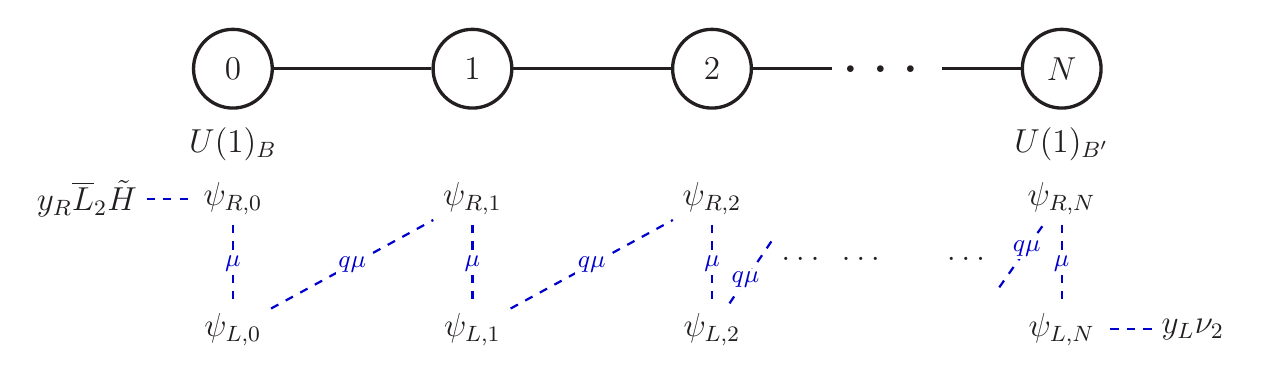
\begin{tikzpicture}[
        node distance=1.5cm and 2cm,
        site/.style={circle, draw, very thick, minimum size=1.0cm, inner sep=0pt, font=\large},
        field/.style={font=\large},
        coupling/.style={blue!80!black, dashed, thick},
        label/.style={fill=white, inner sep=1pt, text=blue!80!black, font=\small}
    ]

    % --- 1. Draw the Theory Space Nodes (Top Row) ---
    \node[site] (n0) {0};
    \node[site, right=of n0] (n1) {1};
    \node[site, right=of n1] (n2) {2};
    
    % Dots for the chain break
    \node[right=1.0cm of n2, font=\Huge] (dots) {$\dots$};
    
    \node[site, right=1.0cm of dots] (nN) {$N$};

    
    \node[field, below=0.1cm of n0] (f0) {$U(1)_{B}$};
    
    \node[field, below=0.1cm of nN] (fN) {$U(1)_{B'}$};

    % Connect the nodes (Theory Space Chain)
    \draw[very thick] (n0) -- (n1);
    \draw[very thick] (n1) -- (n2);
    \draw[very thick] (n2) -- (dots);
    \draw[very thick] (dots) -- (nN);

    % --- 2. Place the Fields (Below Nodes) ---
    % Site 0
    \node[field, below=0.8cm of n0] (r0) {$\psi_{R,0}$};
    \node[field, below=1.0cm of r0] (l0) {$\psi_{L,0}$};

    % Site 1
    \node[field, below=0.8cm of n1] (r1) {$\psi_{R,1}$};
    \node[field, below=1.0cm of r1] (l1) {$\psi_{L,1}$};

    % Site 2
    \node[field, below=0.8cm of n2] (r2) {$\psi_{R,2}$};
    \node[field, below=1.0cm of r2] (l2) {$\psi_{L,2}$};

    %site 2.5
    \node[field, right=0.5cm of r2] (r3){};
    \node[field, below=0.5cm of r3] (m3){$\quad \quad \dots \,\,\, \dots$};
    \node[field, right=0.5cm of l2] (l3){};

    % Site N
    \node[field, below=0.8cm of nN] (rN) {$\psi_{R,N}$};
    \node[field, below=1.0cm of rN] (lN) {$\psi_{L,N}$};

        %site 3.5
    \node[field, left=0.5cm of rN] (r4){};
    \node[field, below=0.5cm of r4] (m4){$\dots$};
    \node[field, left=0.5cm of lN] (l4){};
    % --- 3. Draw Couplings (The "Sawtooth" Pattern) ---
    
    % Vertical Mass Terms (-m L_j R_j)
    \draw[coupling] (r0) -- node[label] {$\mu$} (l0);
    \draw[coupling] (r1) -- node[label] {$\mu$} (l1);
    \draw[coupling] (r2) -- node[label] {$\mu$} (l2);
    \draw[coupling] (rN) -- node[label] {$\mu$} (lN);

    % Diagonal Mixing Terms (-q m_{CW} L_j R_{j+1})
    \draw[coupling] (l0) -- node[label] {$q\mu$} (r1);
    \draw[coupling] (l1) -- node[label] {$q\mu$} (r2);
    
    % For the dots section
    \draw[coupling, shorten >=0.5cm] (l2) -- node[label, near start] {$q\mu$} (r3);
    \draw[coupling, shorten <=0.5cm] (l4) -- node[label, near end] {$q\mu$} (rN);

    % --- 4. External Fields (Input/Output) ---
    
    % SM Lepton Doublet coupling to R_0
    \node[left=0.6cm of r0, font=\large] (L2) {$y_R \overline{L}_2 \tilde{H}$};
    \draw[coupling, thick] (L2) -- (r0);

    % SM Neutrino coupling to L_N
    \node[right=0.6cm of lN, font=\large] (nu2) {$y_L \nu_2$};
    \draw[coupling, thick] (nu2) -- (lN);

    \end{tikzpicture}
    \caption{Schematic representation of the Clockwork chain. The nodes $0 \dots N$ represent sites in theory space. The dashed blue lines represent the mass mixing. The vertical lines correspond to the site-local mass $\mu$, while the diagonal lines represent the nearest-neighbour mixing $q\mu$. The overlap of the zero-mode with the boundary fields generates the suppression $y_{22} \sim q^N$.}
    \label{fig:clockwork_diagram}
\end{figure}
here, the connecting chain consists of $N+1$ right-handed and $N+1$
left-handed fermions and $q<1$, $\mu \sim \Lambda_{\text{FN}}$. The structure of
the Lagrangian in \cref{Clockwork Chain} is preserved by the approximate
$[U(1)]^{N+1}$ symmetry, such that at each node, the fermions $\psi_j$ have
charge $1$ under $U(1)_j$. In this framework, the mass parameter $m$ and the
symmetry-breaking parameter $q$ are treated as background values of spurion
fields, with $q_j$ \bca{What precisely is $q_j$?} having charge $(1,-1)$ under $U(1)_j\times U(1)_{j+1}$ (we
can use a cyclic symmetry to keep the couplings approximately equal
\bca{Why only approximately?}
\cite{arkani-hamed_constructing_2001}). This thereby ensures that
``non-local'' couplings, connecting site$-0$ to site$-N$ directly, are
forbidden, and the Lagrangian remains local in theory space (see
\cref{fig:clockwork_diagram}). The coupling connecting site$-0$ to site$-N$
can only be generated, therefore, by an operator suppressed by a factor of
$q^N$ as shall be shown below. This structure can be viewed as locality in a
discretised extra dimension (the theory space).
\bca{What relates all of these masses? Why aren't they all different parameters?}

To ensure that the suppression of the Yukawa matrix is isolated only to the $Y_{22}$ element, we can label the nodes, $U(1)_I$, such that $L_1, L_2, L_3$ attach to $U(1)_A, U(1)_B, U(1)_C$ and $\nu_1,\nu_2, \nu_3$ to $U(1)_{A'}, U(1)_{B'}, U(1)_{C'}$ with the path/chain length between B and B' being $n(BB')=N+1$ and the rest having a length of one. That is, only $L_2$ and $\nu_2$ are significantly separated in theory space, while the other fields are neighbouring.

For the sake of brevity, we can understand the behaviour by integrating out
the chain using the tree-level equations of motion (EOM), 
\begin{comment}
    \bca{What happened to the derivative
  terms? Also, you've just introduced `EOM': \emph{every} acronym has to be
  defined on the first instance, i.e. equations of motion (EOM).}
\end{comment}

\begin{align}
    \frac{\partial \mathcal{L}}{\partial\overline \psi_{L,k}} = -\mu \psi_{R,k} + \mu q \psi_{R,k+1} + \delta_{N,k}y_L \mu \nu_2 &= 0, \\
    \implies \psi_{R,k} = q^{-k} \psi_{R,0}, \,\,\,\,\,\,\, \psi_{R,N} = y_{L}\nu_2, \\
    \frac{\partial \mathcal{L}}{\partial \psi_{R,k}} = -\mu \overline\psi_{L,k} + \mu q \overline\psi_{L,k-1} + \delta_{0,k}y_R \overline L_2 \tilde{H} &= 0, \\
    \implies\overline\psi_{L,k} = q^{k} \overline\psi_{L,0}, \,\,\,\,\,\,\, \overline\psi_{L,0} = \frac{y_R}{\mu}\overline L_2 \tilde H, 
\end{align}
substituting this into the Lagrangian \cref{Clockwork Chain}, 
\begin{equation}
    \mathcal{L}_{eff} = q^N y_Ry_L \overline L_2\tilde H \nu_2 + \textrm{H.c.},
\end{equation}
where the effective Yukawa coupling is $y_{22} \approx q^N y_L y_R$. For $q<1,
N\gg1$, we get a large suppression, as required by our model to sustain a
normal hierarchy. With $q=0.5, N = 4$, we get a suppression of $0.06$, which
is sufficient to match the $\epsilon^{-4}$ enhancement coming from the
Frogatt-Nielson charge allocation and the seesaw model. \bca{Is this the
  correct criterion?}

A similar setup can be used to explain the texture zeros required to accommodate the inverted neutrino mass hierarchy. The focus, primarily, will be on the bare Majorana matrix $A$ given in \cref{eqn:MajoranaMatrixFact}. This can be extended easily to the case with the mediators to create the Froggatt-Nielson suppression. 

First, looking at the factorization property of $M$,
\begin{equation}
    \label{eqn:MajoranaMatrixFact}
M = M_0 \Sigma A \Sigma, \qquad 
    \Sigma = \begin{pmatrix}
    \epsilon^{1} & 0 & 0 \\
     0 & \epsilon^2 & 0 \\
     0 & 0 & 1 \\
    \end{pmatrix}, \qquad
A =     \begin{pmatrix}
        a_{11} & a_{12}  & a_{13} \\
        a_{12} & a_{22}  & a_{23} \\
        a_{13} & a_{23} & a_{33} 
    \end{pmatrix},
\end{equation} 
we can depict this as shown in \cref{fig:IntCWinFN}. The inter-mediator particles $F_{i}$ have zero $U(1)_X$ charge, but possess the same global symmetries as the corresponding $\nu_i$.
\begin{figure}[t] 
    \centering
    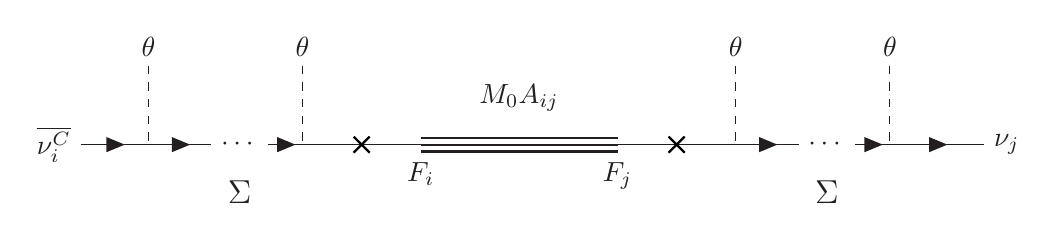
\begin{tikzpicture}
        \begin{feynman}
            % --- LEFT SIDE: \nu_i to F_i (First FN Chain) ---
            \vertex (L) {$\overline{\nu_i^C}$};
            \vertex [right=1.2cm of L] (F1);
            \vertex [above=1.0cm of F1] (phi1) {$\theta$};
            
            % The variable theta insertions
            \vertex [right=0.8cm of F1] (M1) {$\cdots$};
            \vertex [below=0.6cm of M1] {\large $\Sigma$}; % Label for Sigma factor
            
            \vertex [right=0.8cm of M1] (F2);
            \vertex [above=1.0cm of F2] (phi2) {$\theta$};
            
            % Connection to the clockwork gear
            \vertex [right=1.5cm of F2] (Fi_node);
            \vertex [below=0.1cm of Fi_node] {$F_i$};
            
            % Midpoint for the mass insertion cross
            \path (F2) -- (Fi_node) coordinate[midway] (C1); 
            
            % --- MIDDLE: Clockwork Chain (F_i to F_j) ---
            \vertex [right=2.5cm of Fi_node] (Fj_node);
            \vertex [below=0.1cm of Fj_node] {$F_j$};
            
            % Label for Clockwork
            \path (Fi_node) -- (Fj_node) node[midway, above=0.3cm] {$M_0 A_{ij}$}; 
            
            % --- RIGHT SIDE: F_j to \nu_j (Second FN Chain) ---
            \vertex [right=1.5cm of Fj_node] (F3);
            \vertex [above=1.0cm of F3] (phi3) {$\theta$};
            
            % Midpoint for the mass insertion cross
            \path (Fj_node) -- (F3) coordinate[midway] (C2); 
            
            % The variable theta insertions
            \vertex [right=0.8cm of F3] (M2) {$\cdots$};
            \vertex [below=0.6cm of M2] {\large $\Sigma$}; % Label for Sigma factor
            
            \vertex [right=0.8cm of M2] (F4);
            \vertex [above=1.0cm of F4] (phi4) {$\theta$};
            
            \vertex [right=1.2cm of F4] (R) {$\nu_j$};

            % --- DRAWING THE FEYNMAN LINES ---
            \diagram*{
                (L) -- [fermion] (F1) -- [fermion] (M1) -- [fermion] (F2) --  (Fi_node),
                (phi1) -- [scalar] (F1),
                (phi2) -- [scalar] (F2),
                
                (Fj_node) -- (F3) -- [fermion] (M2) -- [fermion] (F4) -- [fermion] (R),
                (phi3) -- [scalar] (F3),
                (phi4) -- [scalar] (F4),
            };

            % --- MANUAL DRAWINGS (Clockwork & Crosses) ---
            
            % 3 parallel lines for the Clockwork Mechanism
            \draw[thick] (Fi_node) -- (Fj_node);
            \draw[thick, transform canvas={yshift=2.5pt}] (Fi_node) -- (Fj_node);
            \draw[thick, transform canvas={yshift=-2.5pt}] (Fi_node) -- (Fj_node);

            % Crosses to show integrating out massive fermions
            \node [cross out, draw=black, thick, minimum size=5pt, inner sep=0pt] at (C1) {};
            \node [cross out, draw=black, thick, minimum size=5pt, inner sep=0pt] at (C2) {};

        \end{feynman}
    \end{tikzpicture}
    \caption{Integrated clockwork chain into the Froggatt-Nielson Mechanism.} \label{fig:IntCWinFN}
\end{figure}

We assume that the fields $\nu_1, \nu_2,\nu_3$ (correspondingly
$F_1,F_2,F_3$), have a negative unit charge under global $U(1)_A, U(1)_B$  and
$U(1)_C$ groups respectively. This forbids the Majorana mass matrix
entirely. To reintroduce the required couplings, we add spurions as before to
the UV spectrum, with the $(U(1)_A,\ U(1)_B,\ U(1)_C)$ charges $(-1,\ 1,\ 0), (0,\ -1,\ 1), (0,\ -2,\ 0),$ and $
  (0,\ 0,\ -2)$. 
\begin{comment}
      \bca{YOu're introducing new notation here and
  must spell it out. I suggest instead: `The $(U(1)_A,\ U(1)_B,\ U(1)_C)$
  charges of the added spurions are (-1,\ 1,\ 0), (0,\ -1,\ 1), (0,\ -2,\ 0),
  (0,\ 0,\ -2).'
}
\end{comment}
With this, we can write down the Lagrangian for direct couplings ($a_{22}$),
\begin{equation} \label{eqn:IOCMdirect}
    \mathcal{L} = a_{0} \overline{\psi_{L0}} F_{2}^C + a_1 \overline{\psi_{R1}} F_2 - \mu(\overline{\psi_{L0}}\psi_{R0} + \overline{\psi_{L1}}\psi_{R1}) + \mu q \overline{\psi_{R1}^C} \psi_{R0} + \textrm{H.c.}
\end{equation}
where we have used the spurion field with charge $(0,-2,0)$. One can now do the
same for the term $a_{33}$, using the spurion with charge $(0,\ 0,\ -2)$. 

For the cross terms, we write,
\begin{equation} \label{eqn:IOCMdiagonal}
    \mathcal{L} = a_{0}' \overline{F_{1}^C} \chi_{R0} + a_1' \overline{\chi_{L1}} F_2  - \mu (\overline{\chi_{L0}}\chi_{R0} + \overline{\chi_{L1}}\chi_{R1}) + \mu q \overline{\chi_{L0}} \, \chi_{R1} + \textrm{H.c.} ,
\end{equation}
where we have used the spurion with charge $(-1,1,0)$. We can do the same
with the coupling of $\nu_2$ to $\nu_3$, where we now use the spurion with
charge $(0,\ -1, 1)$. Now, importantly, since there exists no spurion with
charge $(-1,\ 0,\ 1)$ or $(0,\ 0,\ 2)$, there can be no direct coupling as written in
the Lagrangians \cref{eqn:IOCMdirect} or
\cref{eqn:IOCMdiagonal}. Consequently, the effective couplings $a_{11}$ and $a_{13}$ are generated only at higher orders in the spurion expansion (e.g. via mixing through the $\nu_2$ sector), resulting in the suppression factors $q^m$ and $q^n$, respectively. Using the EOM as before, we can write down an effective Majorana mass matrix of the form,
\begin{equation}
    M_0 A = (M_0 q)
    \begin{pmatrix}
    q^m a_{11}&a_{12}&q^n a_{13}\\
    
    a_{12} &  a_{22}&  a_{23}\\
    
    q^n a_{13} & a_{23}&a_{33} 
    \end{pmatrix}.
\end{equation}
here, the overall factor of $q$ that arises from the spurion couplings as
given in \cref{eqn:IOCMdirect} and \cref{eqn:IOCMdiagonal} has been factored
out of the matrix to multiply the mass scale $M_0$. The couplings $a_{11}$ and
$a_{13}$ come with extra factors of $q$, where $n,m \geq 1$, arising from
indirect (through the $\nu_2$ sector) couplings between $\nu_1$ to $\nu_3$ and
$\nu_1$ to $\nu_1$. For sufficiently small values of $q$, the couplings $a_{11}, a_{13}$ become negligible compared to the rest of the terms, giving us the desired matrix with the texture zeros as in \cref{eqn:IOtexture}. 

\begin{comment}   
\bca{What is `itself'?}
\pcs{\begin{equation}
    \mathcal{L}_{eff} = \langle \Phi_{ij}\rangle \overline{\nu_{i}^C} \nu_j  + \textrm{H.c.} ,
\end{equation}
where $\Phi_{ij}$ can have charges $(-1, 1, 0)$,  $(0, -1, 1)$,  $(0, -2, 0)$ or  $(0, 0, -2)$ in the $(U(1)_A, U(1)_B, U(1)_C)$ space, while the $\nu_i$ are each assigned to the distinct negative unit vectors. and $\langle\Phi\rangle \sim M_0$}

We see that to include the Froggatt-Nielson suppression factors, we can include the mediator chains as depicted in \cref{fig:spag} at the end of the clockwork chains before coupling them back to the RH neutrinos.

\begin{equation} \label{eqn:IOCMdirect}
    \mathcal{L} = a_{0} \overline {\psi _{L0}} \overline{\nu_{2}^C} + a_1 \overline{\psi_{L1}} \nu_2  - m(\overline{\psi_{L0}}\psi_{R0} + \overline{\psi_{L1}}\psi_{R1}) + mq  \overline{\psi_{R1}^C}\psi_{R0} + \textrm{H.c.} ,
\end{equation}

For the inverted hierarchy case, we use a similar setup with the Lagrangian,
\begin{equation} \label{Clockwork Chain}
    \mathcal{L} = -m\sum_{j = 0}^{N-1} (\overline \psi_{L,j}\psi_{R,j} - q\overline \psi_{L,j} \psi_{R,j+1}) - m\overline\psi_{L,N}\psi_{R,N} + A_1 \overline {\nu_{R1}^c} \psi_{R, 0} + A_2  \overline \psi_{L, N} \nu_3 + \textrm{H.c.},
\end{equation}

\end{comment}

\bibliographystyle{JHEP-2}
\bibliography{article}


\end{document}
